% Chapter 6
\section*{Preface}
In this chapter, performance of AIBs using various kinds of materials was explored. Nanostructured molybdenum dichalcogenides (\ce{MoS2} and \ce{MoSe2}), graphitic carbon nitride (g-\ce{C3N4}), and electrospun tin oxide \ce{SnO2} fibers were tested as cathodes and their results have been reported. Prussian blue, which is a three-dimensional (3D) metal-organic framework (MOF), was also investigated as a cathode material. The most successful cathodes have been reported previously in Chapter 4 and 5. The other materials tested as cathodes have been summoned in this chapter. 
\pagebreak
\chapter{Aluminium batteries using various 2D/3D materials as cathodes} 
\label{chap6} 
Recent development in the field of two-dimensional (2D) materials has shown a lot of potential in the field of energy storage. Materials like graphene and its analogues, have remarkable electrochemical properties. They can be used in most of the energy storage devices such as batteries, supercapacitors, redox flow batteries, photovoltaics etc. In addition to their tunable chemical and physical properties, 2D materials possess different crystallographic structures and elemental compositions. For this reason, they find immense use as electrode materials in electrochemical energy storage devices\cite{wang_graphene_2009,bonaccorso_graphene_2015}. Furthermore, graphene and other 2D nanomaterials have a larger theoretical gravimetric capacity \cite{zhou_progress_2014}. 

\begin{figure}[h!]
  \centering
  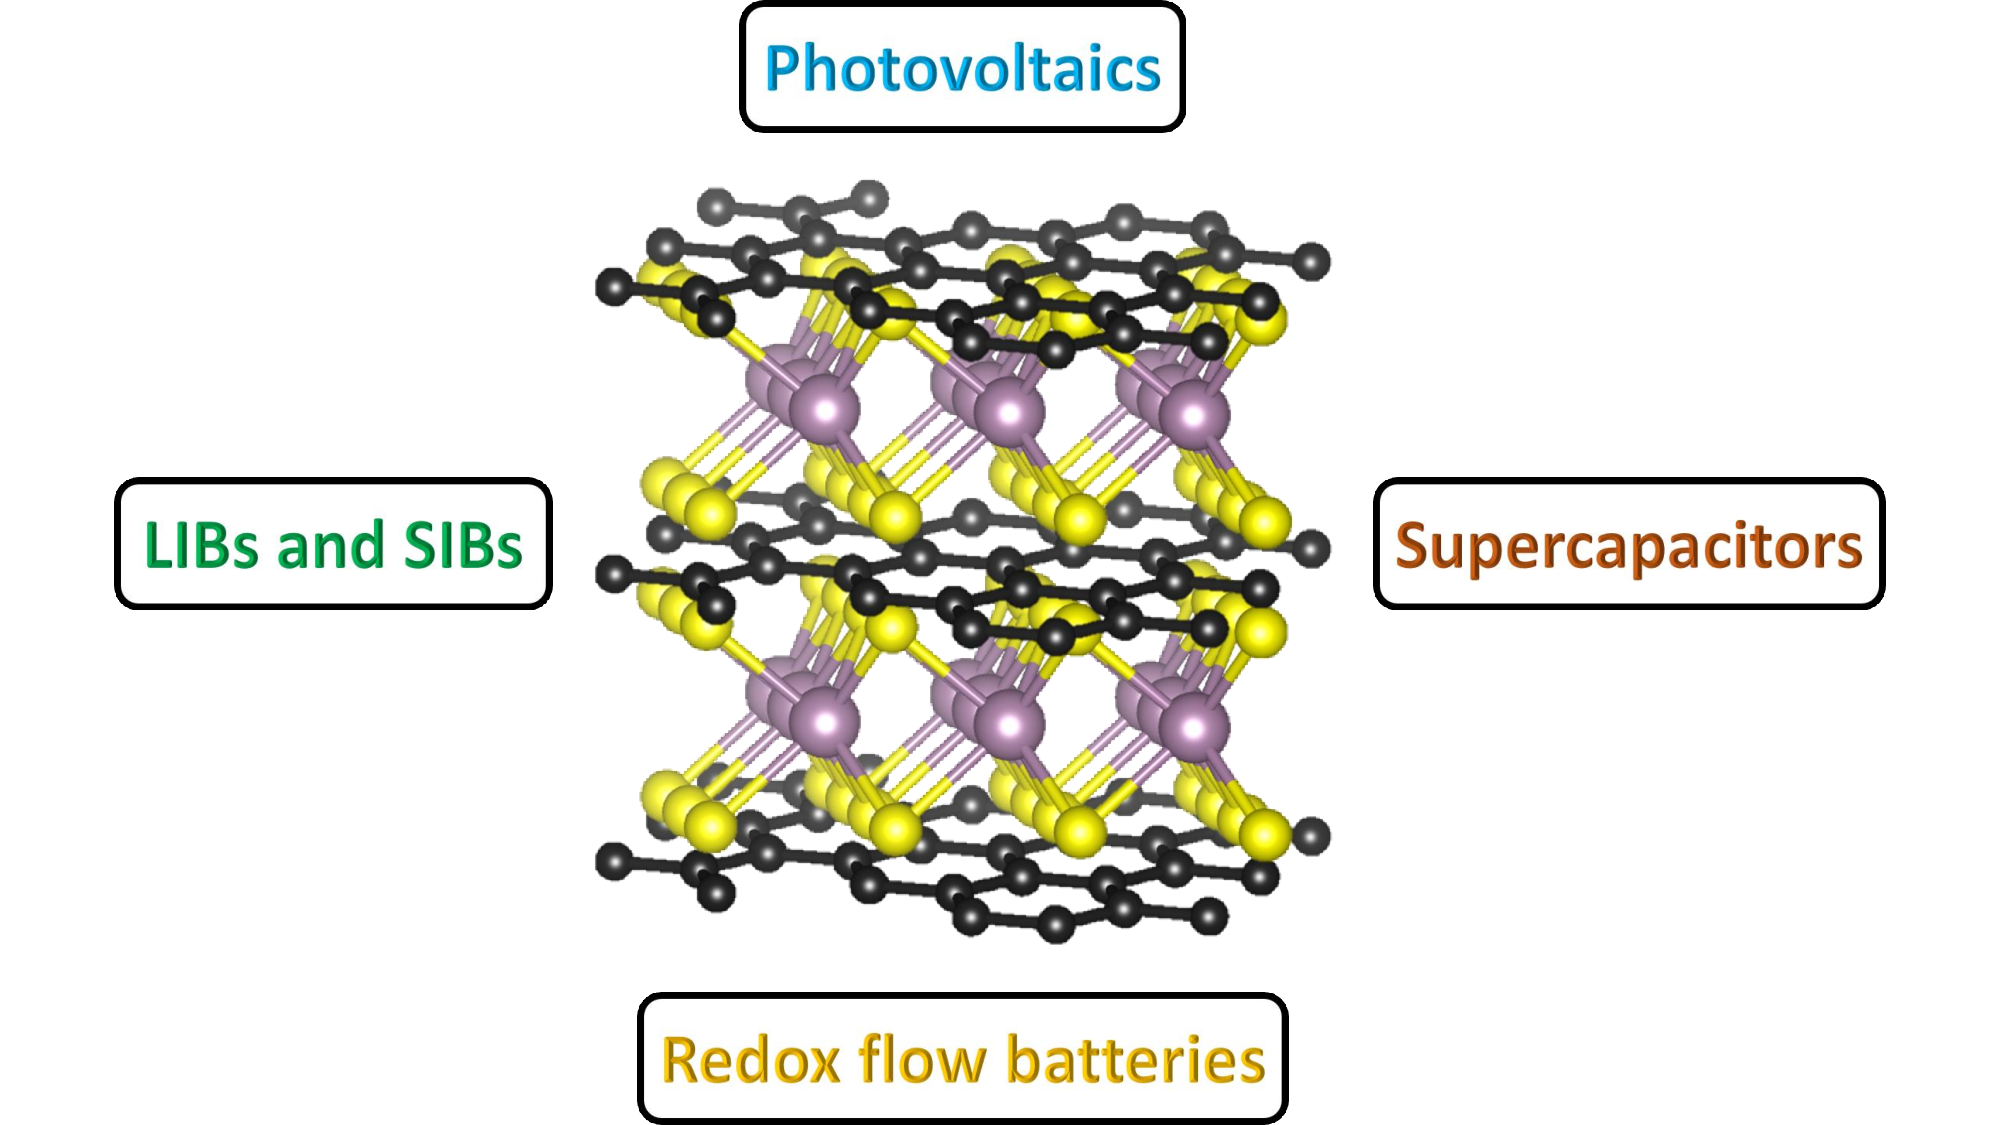
\includegraphics[width=\textwidth]{Figures/chap6fig/nanoTMDintro.pdf}
    \caption{An illustration of various applications of graphene and its analogues such as nanostructured \ce{MoS2}.}
  \label{Figures/chap6fig:nanoTMDintro}
\end{figure}

\section{Nanostructured molybdenum sulfide and selenide}
Some transition metal dichalcogenides (TMDs) such as \ce{TiS2} and exfoliated \ce{MoS2} flakes exhibit fast ionic conductivity as an electrochemically active material \cite{du_superior_2010,whittingham_electrical_1976}. A $\sim$750mAh g$^{-1}$ specific capacity was reported for restacked \ce{MoS2} single layers as a lithium-ion battery electrode. The restacking enlarged the c-axis parameter, which denotes its interlayer spacing, and consequently increased the accessible surface area \cite{ammundsen_novel_2001}.\\
Nanosized materials increase the contact area between an electrode and the electrolyte. They provide shorter path lengths for both ion diffusion and electron transport in comparison with bulk particles. As a result, the charge/ discharge rate is improved. Since a shorter path length for electronic transport is created, materials having low electronic conductivity can also be utilised \cite{pitchai_nanostructured_2011}. The high surface area of nanomaterials allows large volume expansion/ contraction associated with ion intercalation/ de-intercalation and prevents cathode pulverisation, which leads to a longer cycle-life \cite{zhang_ultrathin_2015, cong_intrinsic_2015}. TMDs have the potential to undergo redox reactions because of their multiple oxidation states. Nano TMDs have been widely explored as electrode materials since they have the potential to improve the electrochemical performance. 
These materials have shown some remarkable performances in LIBs, sodium-ion batteries (SIBs), lithium-sulphur (Li-S) batteries, magnesium-ion batteries (MIBs), etc \cite{xie_mos2/graphene_2015,cao_preparation_2013,dong_insights_2019,li_rechargeable_2018}. Nanostructured \ce{MoS2} has been established as a promising material to be used for energy storage. Xie and group synthesised a \ce{MoS2}/ reduced graphene oxide (rGO) nanocomposites as an anode for SIBs \cite{xie_mos2/graphene_2015}. The drawback of these cells was the volume change during charge/discharge cycles. The capacity retention for the nanocomposite with highest \ce{MoS2} ratio was the poorest after 100 cycles. This was attributed to the insufficient amount of rGO, which should have allowed significant volume change during the cycles and store more \ce{Na+} ions. In 2013, Cao \textit{et al.} used \ce{MoS2} coated 3D graphene network (\ce{MoS2}/3DGN) as a binder-free anode material in LIBs \cite{cao_preparation_2013}. The 3DGN improved the electrical contact between the current collector and deposited \ce{MoS2}. The cell displayed a discharge capacity of 466 mAh g$^{-1}$ after 10 cycles at a  high current density of 4 A g$^{-1}$. The lithiation process was accompanied by a phase transformation of \ce{Li_xMoS2} from 2H to 1T during first discharge cycle. To determine the significance of the \ce{MoS2} nanoparticles, another composite using bulk-\ce{MoS2} was prepared. It was observed that due to poor electrical contact between \ce{MoS2} and 3D-GN, the cell underwent rapid capacity decay. This confirmed that the graphene network provided an efficient pathway for \ce{Li+} exchange. It also showed that the nanostructured \ce{MoS2} had more active edge sites than bulk \ce{MoS2}, which resulted in high-performing LIBs. Based on similar principle, Dong \textit{et al.} used \ce{MoS2} nanosheets as an anode material for potassium-ion batteries. They suggested that highly crystalline-\ce{MoS2} displayed higher discharge capacity that poorly-crystallised \ce{MoS2} \cite{dong_insights_2019}. \ce{MoS2} microspheres were used as cathodes in non-aqueous AIBs by Li \textit{et al} \cite{li_rechargeable_2018}. The cell achieved a capacity of 66.7 mAh g$^{-1}$ after 100 cycles at a current rate of 40 mA g$^{-1}$. They found that intercalation of \ce{Al^{3+}} ions into \ce{MoS2} was accompanied by a phase transformation at the electrode interface. It was suggested that formation of a solid electrolyte interface (SEI) layer changed the microstructure of \ce{MoS2}. Furthermore, the cell failed to deliver a stable performance due to electrochemical polarization of \ce{MoS2}. Irreversible capacity losses and low CEs were also reported for this battery. With the rapid progress in research on 2D nanomaterials, large-scale preparation of nanostructured materials at a low cost can be expected for practical applications in the near future. It has been reported that mixing transition metal oxides with nano forms of carbon improves their electrochemical performance in energy storage devices \cite{acerce_metallic_2015-1,zhao_flexible_2015,hu_hierarchical_2015,cao_preparation_2013,ding_facile_2012}. For e.g. \ce{TiO2} displayed a capacity of 182 mAh g$^{-1}$ and retained 88\% of its CE after 400 cycle. The capacity increased to 320 mAh g$^{-1}$ when \ce{TiO2} was mixed with CNT. The cell retained 94\% of its CE after 120 cycles. Table \ref{tmc} compares the performance of transition metals and the metal-nano carbon composites. 

\begin{sidewaystable}
\centering
\caption{Summary of performances of 2D materials in various energy storage devices.} \label{tmc}
\begin{tabular}{ |p{1.5cm}|p{3.5cm}|p{4.5cm}|p{4.5cm}|p{4.5cm}|}
 \hline 
\textbf{Ref.} & \textbf{Electrode} & \textbf{Electrolyte} & \textbf{Storage capacity} & \textbf{Cycle performance} \\ 
\hline
\cite{acerce_metallic_2015-1} & {Supercapacitors: Metallic 1T \ce{MoS2}} & 0.5M \ce{H2SO4}, \ce{Li2SO4}, \ce{K2SO4} or KCl or EMIm \ce{BF4} & Volumetric capacitance: 400-700 F cm$^{-3}$ & >90\% retained after 5000 cycles\\
\cite{zhao_flexible_2015} & Supercapacitors: MXene/CNTs & 1M \ce{MgSO4} & Volumetric capacitance: 350F cm$^{-1}$ & No degradation after 10000 cycles at 10 A g$^{-1}$\\
\cite{hu_hierarchical_2015} & LIB: \ce{TiO2} & 1M \ce{LiPF6} in a 1: (v:v) mixture of ethylene carbonate and dimethyl carbonate & Specific capacity: 182 mAh g$^{-1}$ at 5C & 87.9\% retained after 400 cycles at 5C \\
\cite{cao_preparation_2013} & LIB: \ce{MoS2}/graphene & 1M \ce{LiPF6} in a 1:1 (V:v) mix of ethylene carbonate and dimethyl carbonate & Specific capacity: 466 mAh g$^{-1}$ at 4 A g$^{-1}$ & 566 mAh g$^{-1}$ retained after 50 cycles at 0.5 A g$^{-1}$ \\
\cite{ding_facile_2012} & LIB: \ce{TiO2}/CNT \ce{SnO2}/CNT & 1M \ce{LiPF6} in a 1:1 (w:w) mix of ethylene carbonate and dimethyl carbonate & Specific capacity: 320 mAh g$^{-1}$ for \ce{TiO2}, 580 mAh g$^{-1}$ for \ce{SnO2} at 0.4 A g$^{-1}$ & 93.8\% retained after 120 cycles for \ce{TiO2}, 72.4\% retained after 40 cycles at 0.4 A g$^{-1}$ for \ce{SnO2}\\
\cite{xie_mos2/graphene_2015} & SIB: \ce{MoS2}/rGO & 1M \ce{NaClO4} in a 1:1 (V:v) mix of ethylene carbonate and dimethyl carbonate & Specific capacity: 350 mAh g$^{-1}$ at 0.64 A g$^{-1}$ & 227 mAh g$^{-1}$ retained after 300 cycles at 0.32 A g$^{-1}$ \\
\hline
\end{tabular}
\end{sidewaystable}

\subsection{Experimental methods}
The materials were obtained from Tohoku university and used as received. 
%Before adding sulfur, pristine \ce{MoO3} (Wako chemicals) was ball-milled for 4 hours. 1 mmol of ascorbic acid (Wako chemicals) as a reducing agent was dissolved in 5 ml of water and the mixture was magnetically stirred for at least 20 minutes under air. Subsequently, 1 mmol of S powder (Sigma-Aldrich) and 0.3 mmol of ball-milled \ce{MoO3} were placed in the reactor. Lastly, 5 ml of ascorbic acid aqueous solution was injected into the reactor vessels containing the powder mixture. The sealed reactor was kept at 400$^{\circ}$C in a tube furnace for 30 minutes. After heating, the samples were collected in the same procedure as above.

\subsection{Results and discussion}
In this chapter \ce{MoS2} and \ce{MoSe2} nanoflowers were used as cathodes in non-aqueous AIBs. The \ce{MoS2} and \ce{MoSe2} cells displayed a capacity of 58 and $\sim$100 mAh g$^{-1}$ at a current rate of 50 mAh g$^{-1}$ after 5 and 10 cycles respectively cycles. The performance was significantly better that previously reported bi Li and his group \cite{li_rechargeable_2018}. Figures \ref{Figures/chap6fig:mose2yncdcce} and \ref{Figures/chap6fig:mos2yncdcce} show the charge/ discharge curves and CEs of the cells with cutoff voltages at 0.2 and 2.35 V. It was observed that the discharge curves for both \ce{MoSe2} and \ce{Mos2} looked similar to their bulk counterparts, shown in Figure \ref{Figures/chap6fig:mox2bulkcdccv}a and b. Nano-\ce{MoSe2} displayed discharge voltage plateaus at 1.9 V. There was also a visible voltage bend during discharge at 0.75 V. A plateau was observed during charge at 2.0 V (similar to bulk \ce{MoSe2} seen in Figure \ref{Figures/chap6fig:mox2bulkcdccv}b). In Figure \ref{Figures/chap6fig:mox2yncv}a the CV curves for \ce{MoSe2} displayed redox peaks at potentials corresponding to the voltage plateaus in the charge and discharge curves confirming the presence of redox couples and possibility of ion intercalation. The discharge capacity of nano-\ce{MoSe2} decreased from 90 to 60 mAh g$^{-1}$ after 10 cycles. It seemed the nanostructured \ce{MoSe2} was unable to store charge reversibly unlike its bulk counterpart. Interestingly, the CE of both materials was low at $\sim$40-50\%. This meant that the total charge extracted from the cells was lower than the charge put into them over a full cycle; not all ions that were inserted into the layers were extracted out. Low CE also indicates presence of side reactions. The behaviour of nano-\ce{MoS2} was similar to bulk-\ce{MoS2}. Voltage bends at 2.1 and 0.65 V were observed during discharge (compare Figure \ref{Figures/chap6fig:mos2yncdcce}a and Figure \ref{Figures/chap6fig:mox2bulkcdccv}a). However, the redox peaks present in the voltammogram did not display any redox peaks, unlike bulk-\ce{Mos2} as seen in Figure \ref{Figures/chap6fig:mox2bulkcdccv}c. It was possible that the nano dimensions did not allow reversible intercalation/ de-intercalation to take place. The schematic of a plausible mechanism is illustrated in Figure \ref{Figures/chap6fig:nanbulkmox2}. More ions were now available for surface adsorption rather than ion intercalation. 

\begin{figure}[h!]
  \centering
  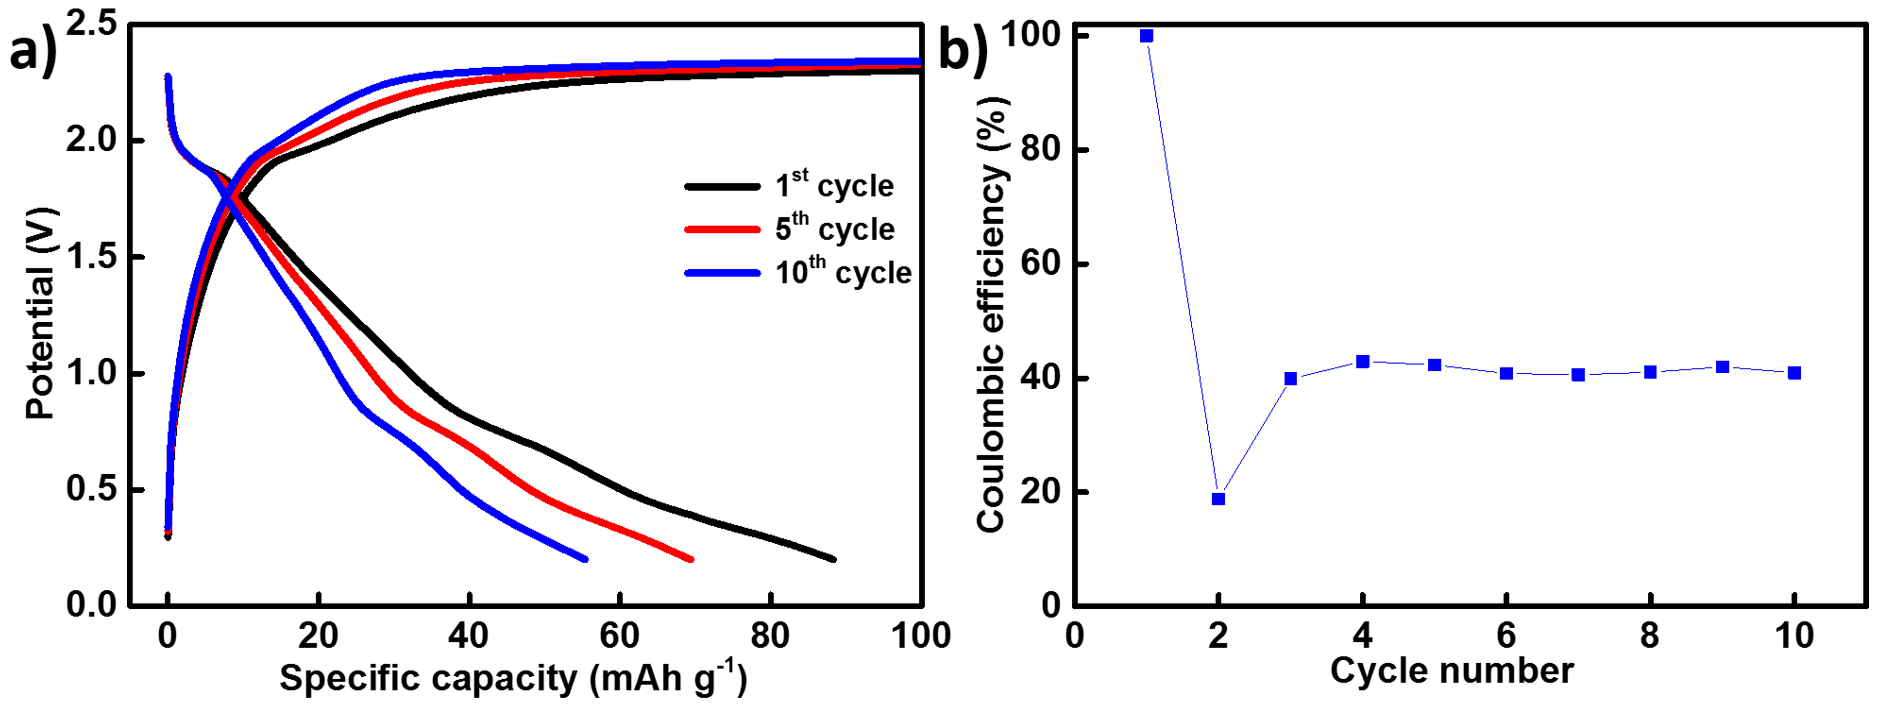
\includegraphics[width=\textwidth]{Figures/chap6fig/mose2yncdcce}
    \caption{Galvanostatic charge and discharge curves of a) Al/\ce{MoSe2} and b) CE for every cycle.}
  \label{Figures/chap6fig:mose2yncdcce}
\end{figure}

\begin{figure}[th!]
\centering

\includegraphics[width=\textwidth]{Figures/chap6fig/mox2yncv}
\caption{Cyclic voltammograms of a)\ce{MoSe2} and b)\ce{MoS2} nanoflowers at the scan rate of 10 mV s$^{1}$.}
\label{Figures/chap6fig:mox2yncv}
\end{figure}

\begin{figure}[h!]
  \centering
  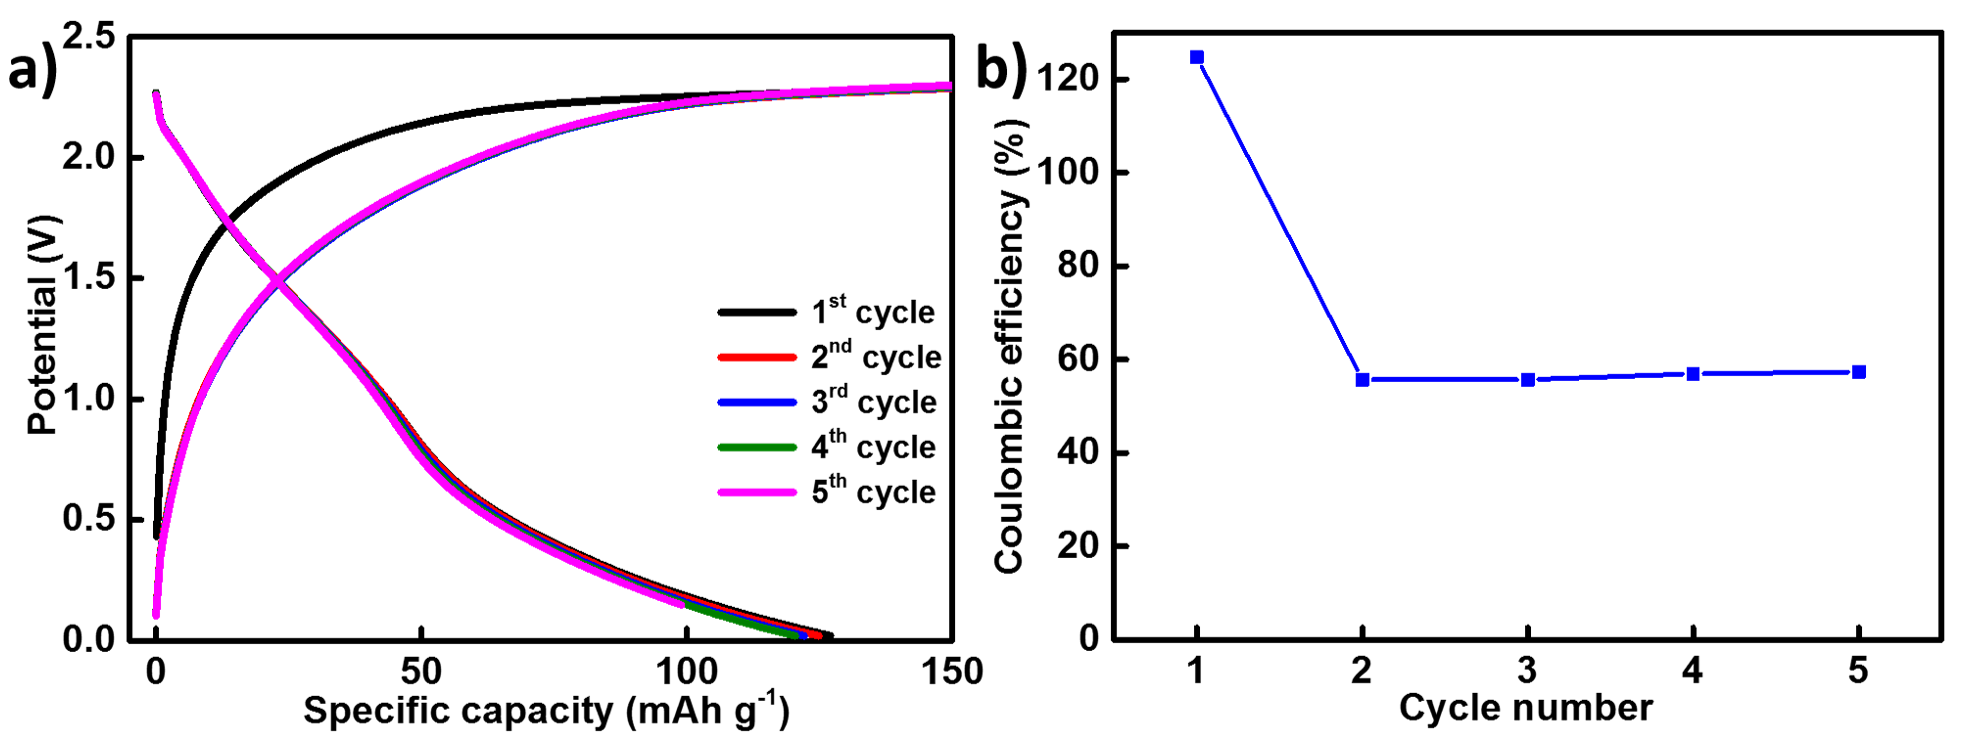
\includegraphics[width=\textwidth]{Figures/chap6fig/mos2yncdcce}
    \caption{Galvanostatic charge and discharge curves of a) Al/\ce{MoS2} and b) CE for every cycle.}
  \label{Figures/chap6fig:mos2yncdcce}
\end{figure}

\begin{figure}[h!]
  \centering
  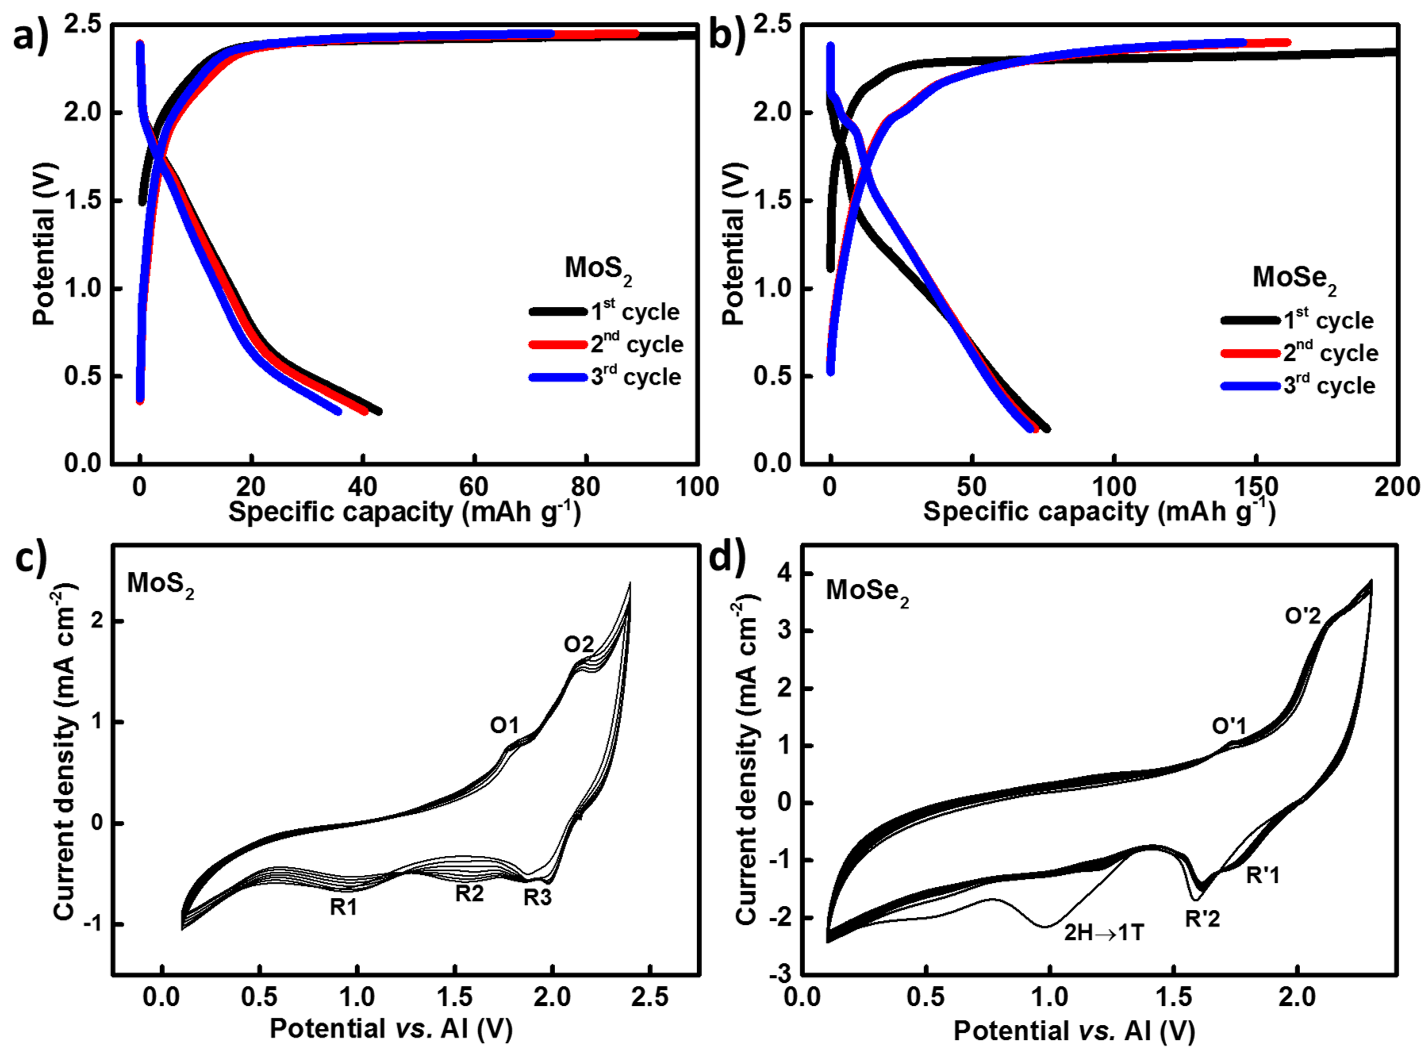
\includegraphics[width=\textwidth]{Figures/chap6fig/mox2bulkcdccv}
    \caption{Galvanostatic charge and discharge curves of a) bulk Al/\ce{MoS2} and b) bulk \ce{MoSe2} cell at a current rate of 50 mA g$^{-1}$. CV scans of bulk c) \ce{MoS2} and d) \ce{MoSe2} with distinct redox peaks marked .}
  \label{Figures/chap6fig:mox2bulkcdccv}
\end{figure}

\begin{figure}[h!]
  \centering
  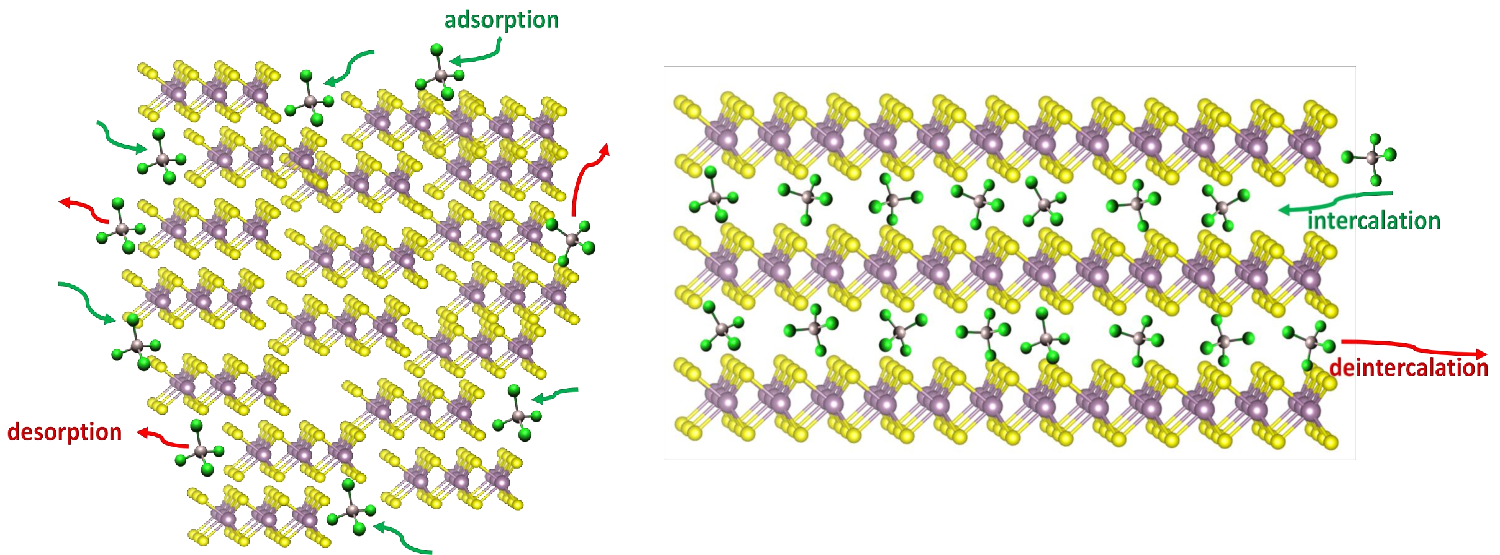
\includegraphics[width=\textwidth]{Figures/chap6fig/nanbulkmox2.pdf}
    \caption{Schematic illustration of charge storage by \ce{MoX2} nanoflowers (left) and bulk material (right). The }
  \label{Figures/chap6fig:nanbulkmox2}
\end{figure}

\subsection{Future outlook}
The nanomaterials used in this chapter might behave differently if:
\begin{itemize}
    \item New nanocomposites are made using carbon-based materials (rGO, CNTs), which would not only improve the contact between the current collector and the active material, but also enhance the cell's capacity by phase transformation, which was missing in the nanoflowers
    \item Increasing the number of layers present; the nanoflowers tested above have very few layers, which might have resulted in faster agglomeration of the active material resulting low cell efficiencies and low discharge capacities. The number of layers can be increased by modifying the synthesis procedure. 
\end{itemize}

\section{Tin oxide}

\subsection{Introduction}

\begin{figure}[th!]
  \centering
  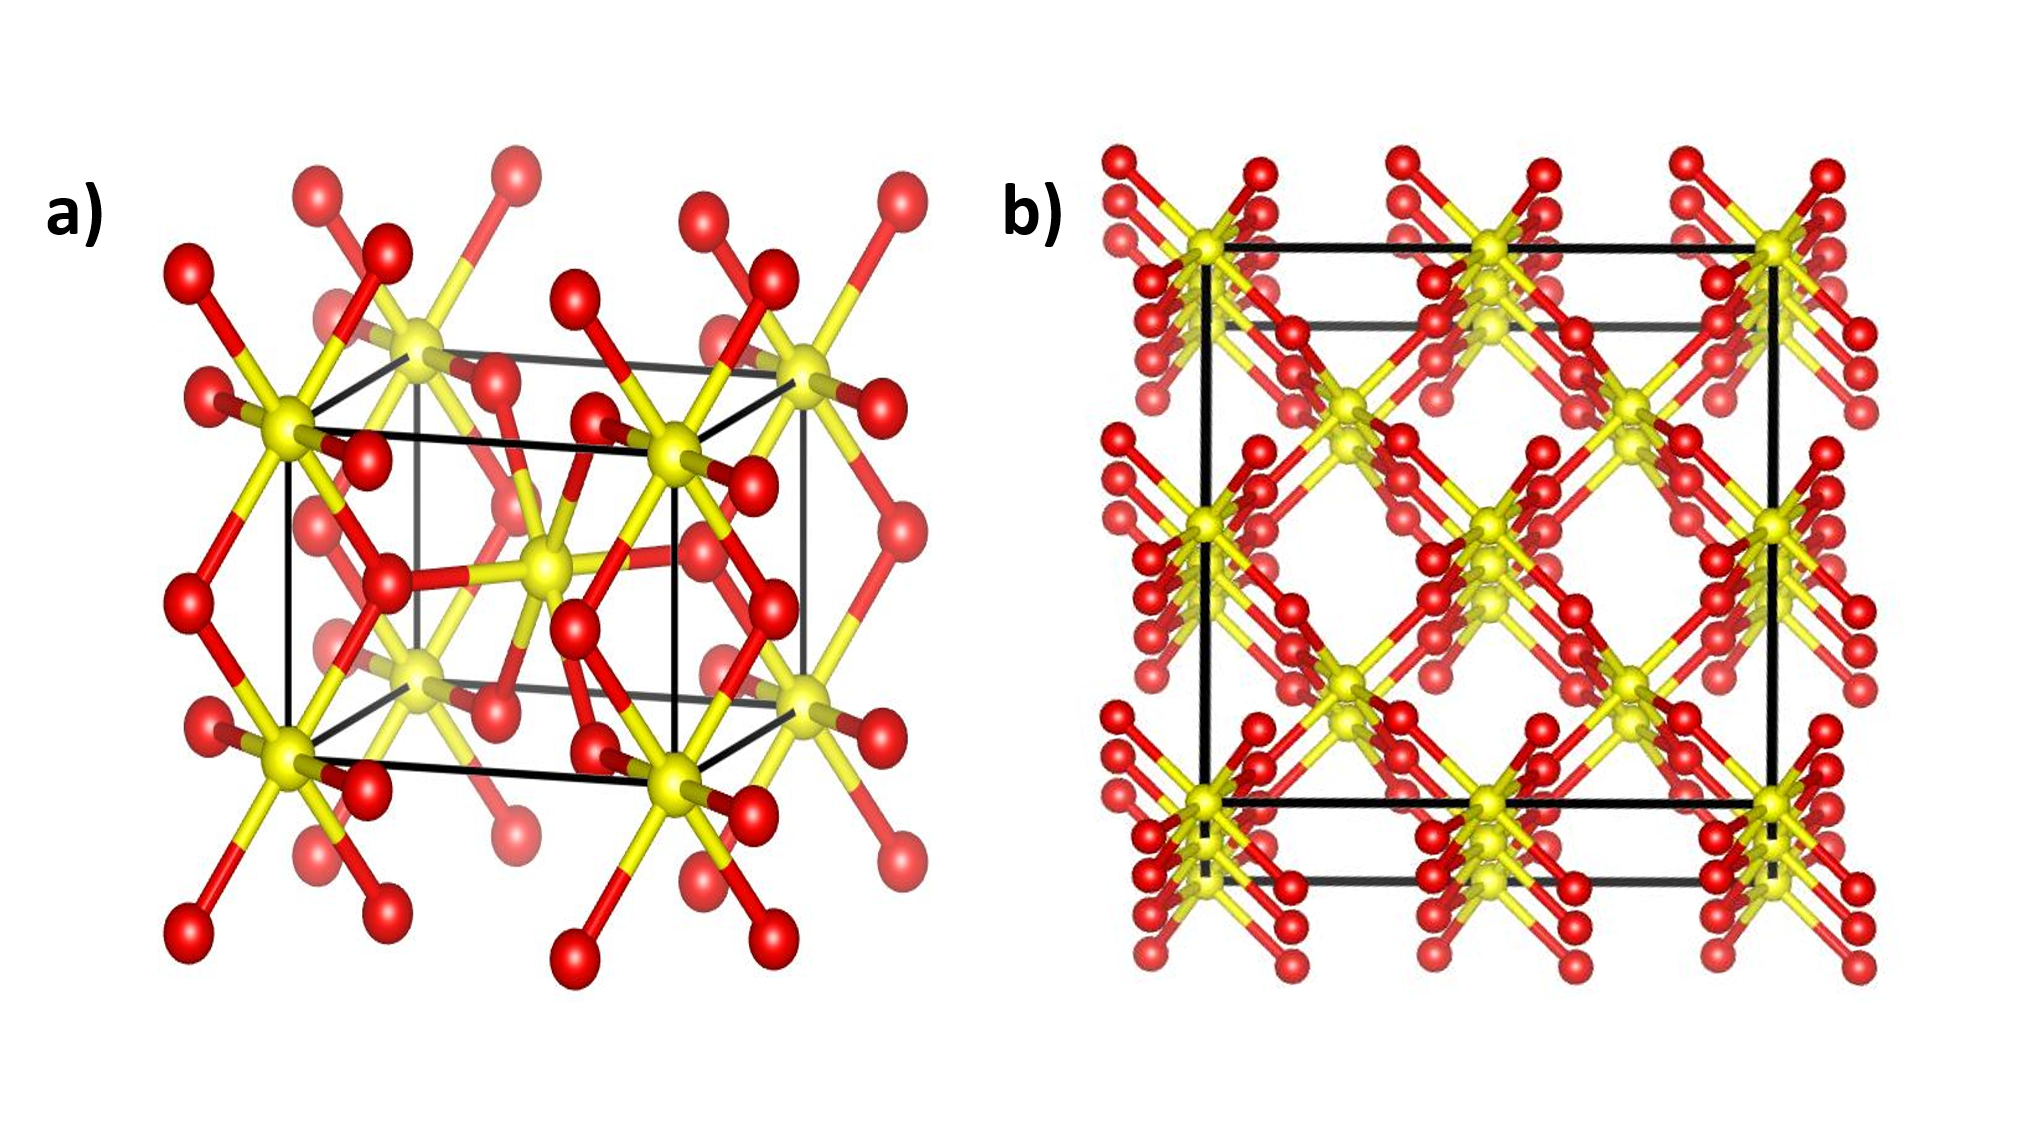
\includegraphics[width=\textwidth]{Figures/chap6fig/SnO2crys}
    \caption{Crystal structure of \ce{SnO2}. Tetragonal unit cell with space group \textit{P4/nmm} and space group number 129.}
  \label{Figures/chap6fig:SnO2crys}
  \end{figure}
  
Due to its high theoretical capacity ($\approx$ 782mAh g$^{-1}$) and safe handling, \ce{SnO2} has been a popular choice as anodes in LIBs  \cite{idota_tin-based_1997}. Unfortunately, the major disadvantage of these materials is the large volume change during lithium insertion/extraction. A volume change of $\sim$360\% in pure tin metal causes an internal strain. Whittingham \textit{et al.} showed that pure tin foil (bulk) can be cycled at 600 mAh g$^{-1}$ for 10 to 15 cycles \cite{yang_anodes_2003}. However, the expansion and contraction of the anode during the cycles causes anode pulverisation and increases of the cell impedance. Consequently, due to the loss of electronic contact between the active material and the current collector, the capacity of the cells decreases after 15 cycles. In some cases, formation of \ce{Li2O} in addition to volume expansion, further deteriorates the battery performance \cite{zhao_tin-based_2016}. Equation 1 describes the formation of \ce{Li2O} and Equation 2 describes the large volume variation that takes place due to formation of \ce{Li_{x}Sn} after Li atom reacts with Sn produced in Equation \cite{park_effect_2008}.

\begin{equation}
\ce{SnO2 + 4Li+ + 4e- -> 2Li2O + Sn} 
\end{equation}
\begin{equation}
x\ce{Li + xe- + ySn -> Li_{x}Sn} 
\end{equation}

Since \ce{Li2O} is electrochemically inactive and non-conductive, it is also responsible for the large initial irreversible capacity. It has been reported that \ce{Li2O} can be decomposed via structural modifications of \ce{SnO2} on a nanoscale. Tin-based anodes have demonstrated improved electrochemical performance and cycle life and a controlled expansion process during lithiation.  

\begin{figure}[th!]
\centering
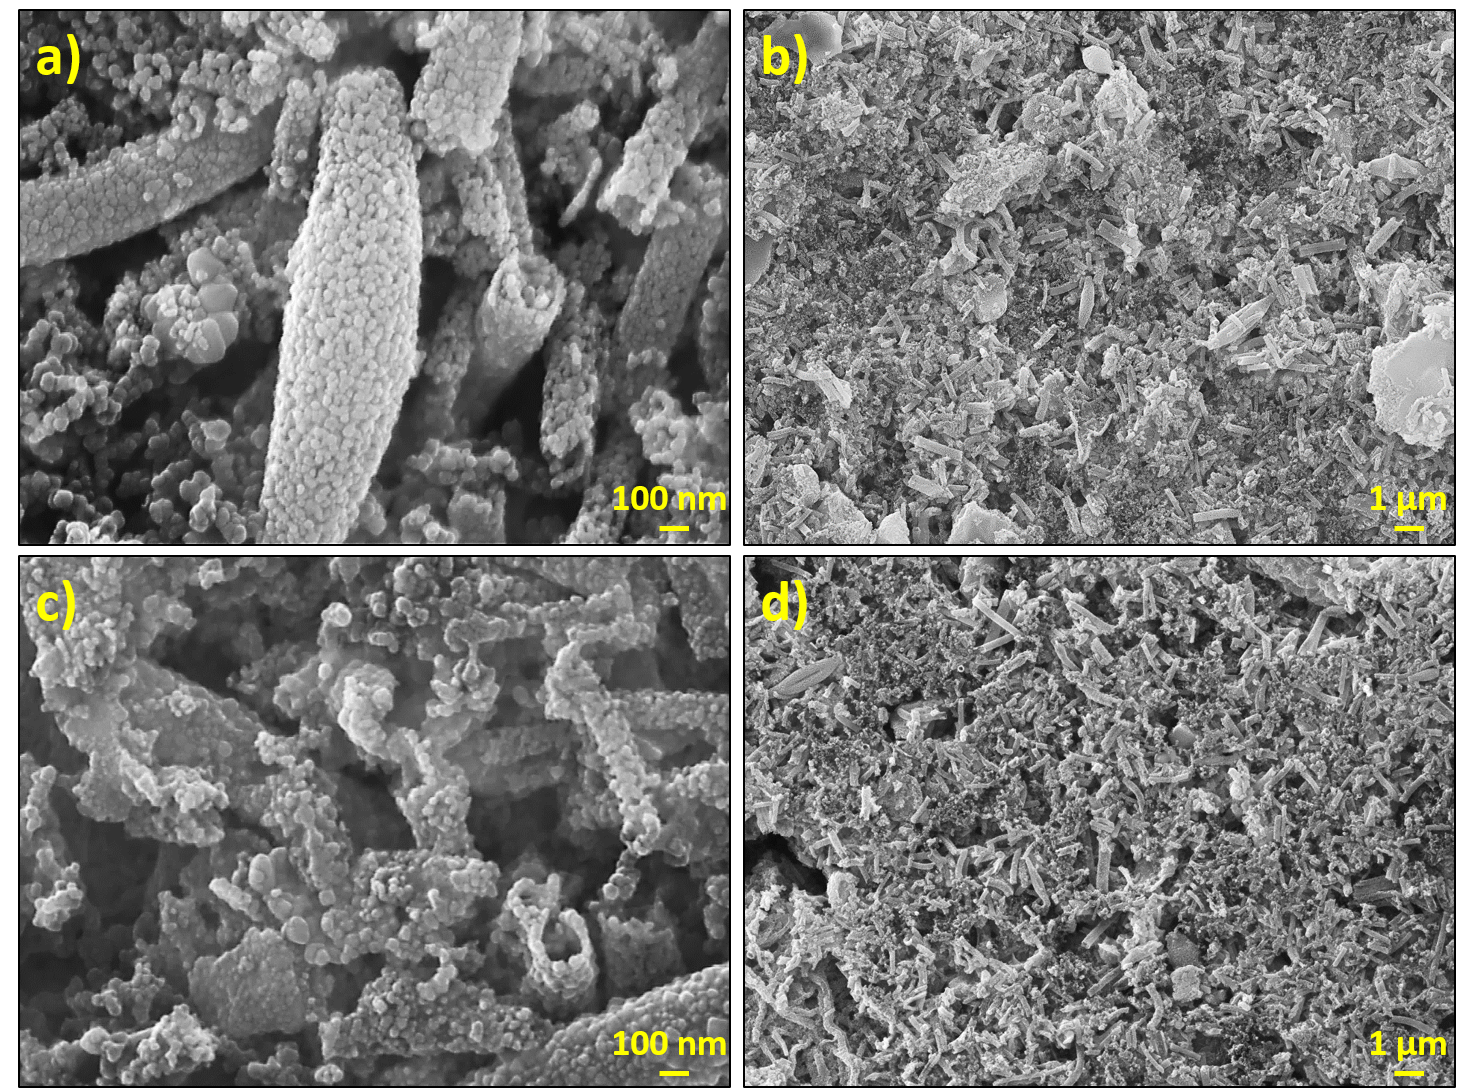
\includegraphics[width=\textwidth]{Figures/chap6fig/SnO2SEM}
\caption{SEM images of a,c)pristine and b,d) cycled \ce{SnO2} cathode.}
\label{Figures/chap6fig:SnO2SEM}
\end{figure}

It has been proposed that adding carbonaceous materials to \ce{SnO2} increases its surface area, which makes more active sites available for lithiation \cite{navarrosuarez_2d_2018}. It also controls the volume expansion/shrinkage. Furthermore, it improves the conductivity of the material \cite{nowak_composites_2018}. Several nanostructured tin-based materials such as nanorods \cite{liu_direct_2009}, nanobelts \cite{duan_single_2005}, nanowires \cite{huang_situ_2010}, nanotubes \cite{wang_large-scale_2011} have been synthesised and tested as electrodes. In this chapter, \ce{SnO2} fibers were obtained via  \enquote{electrospinning}. 

\begin{figure}[th!]
\centering
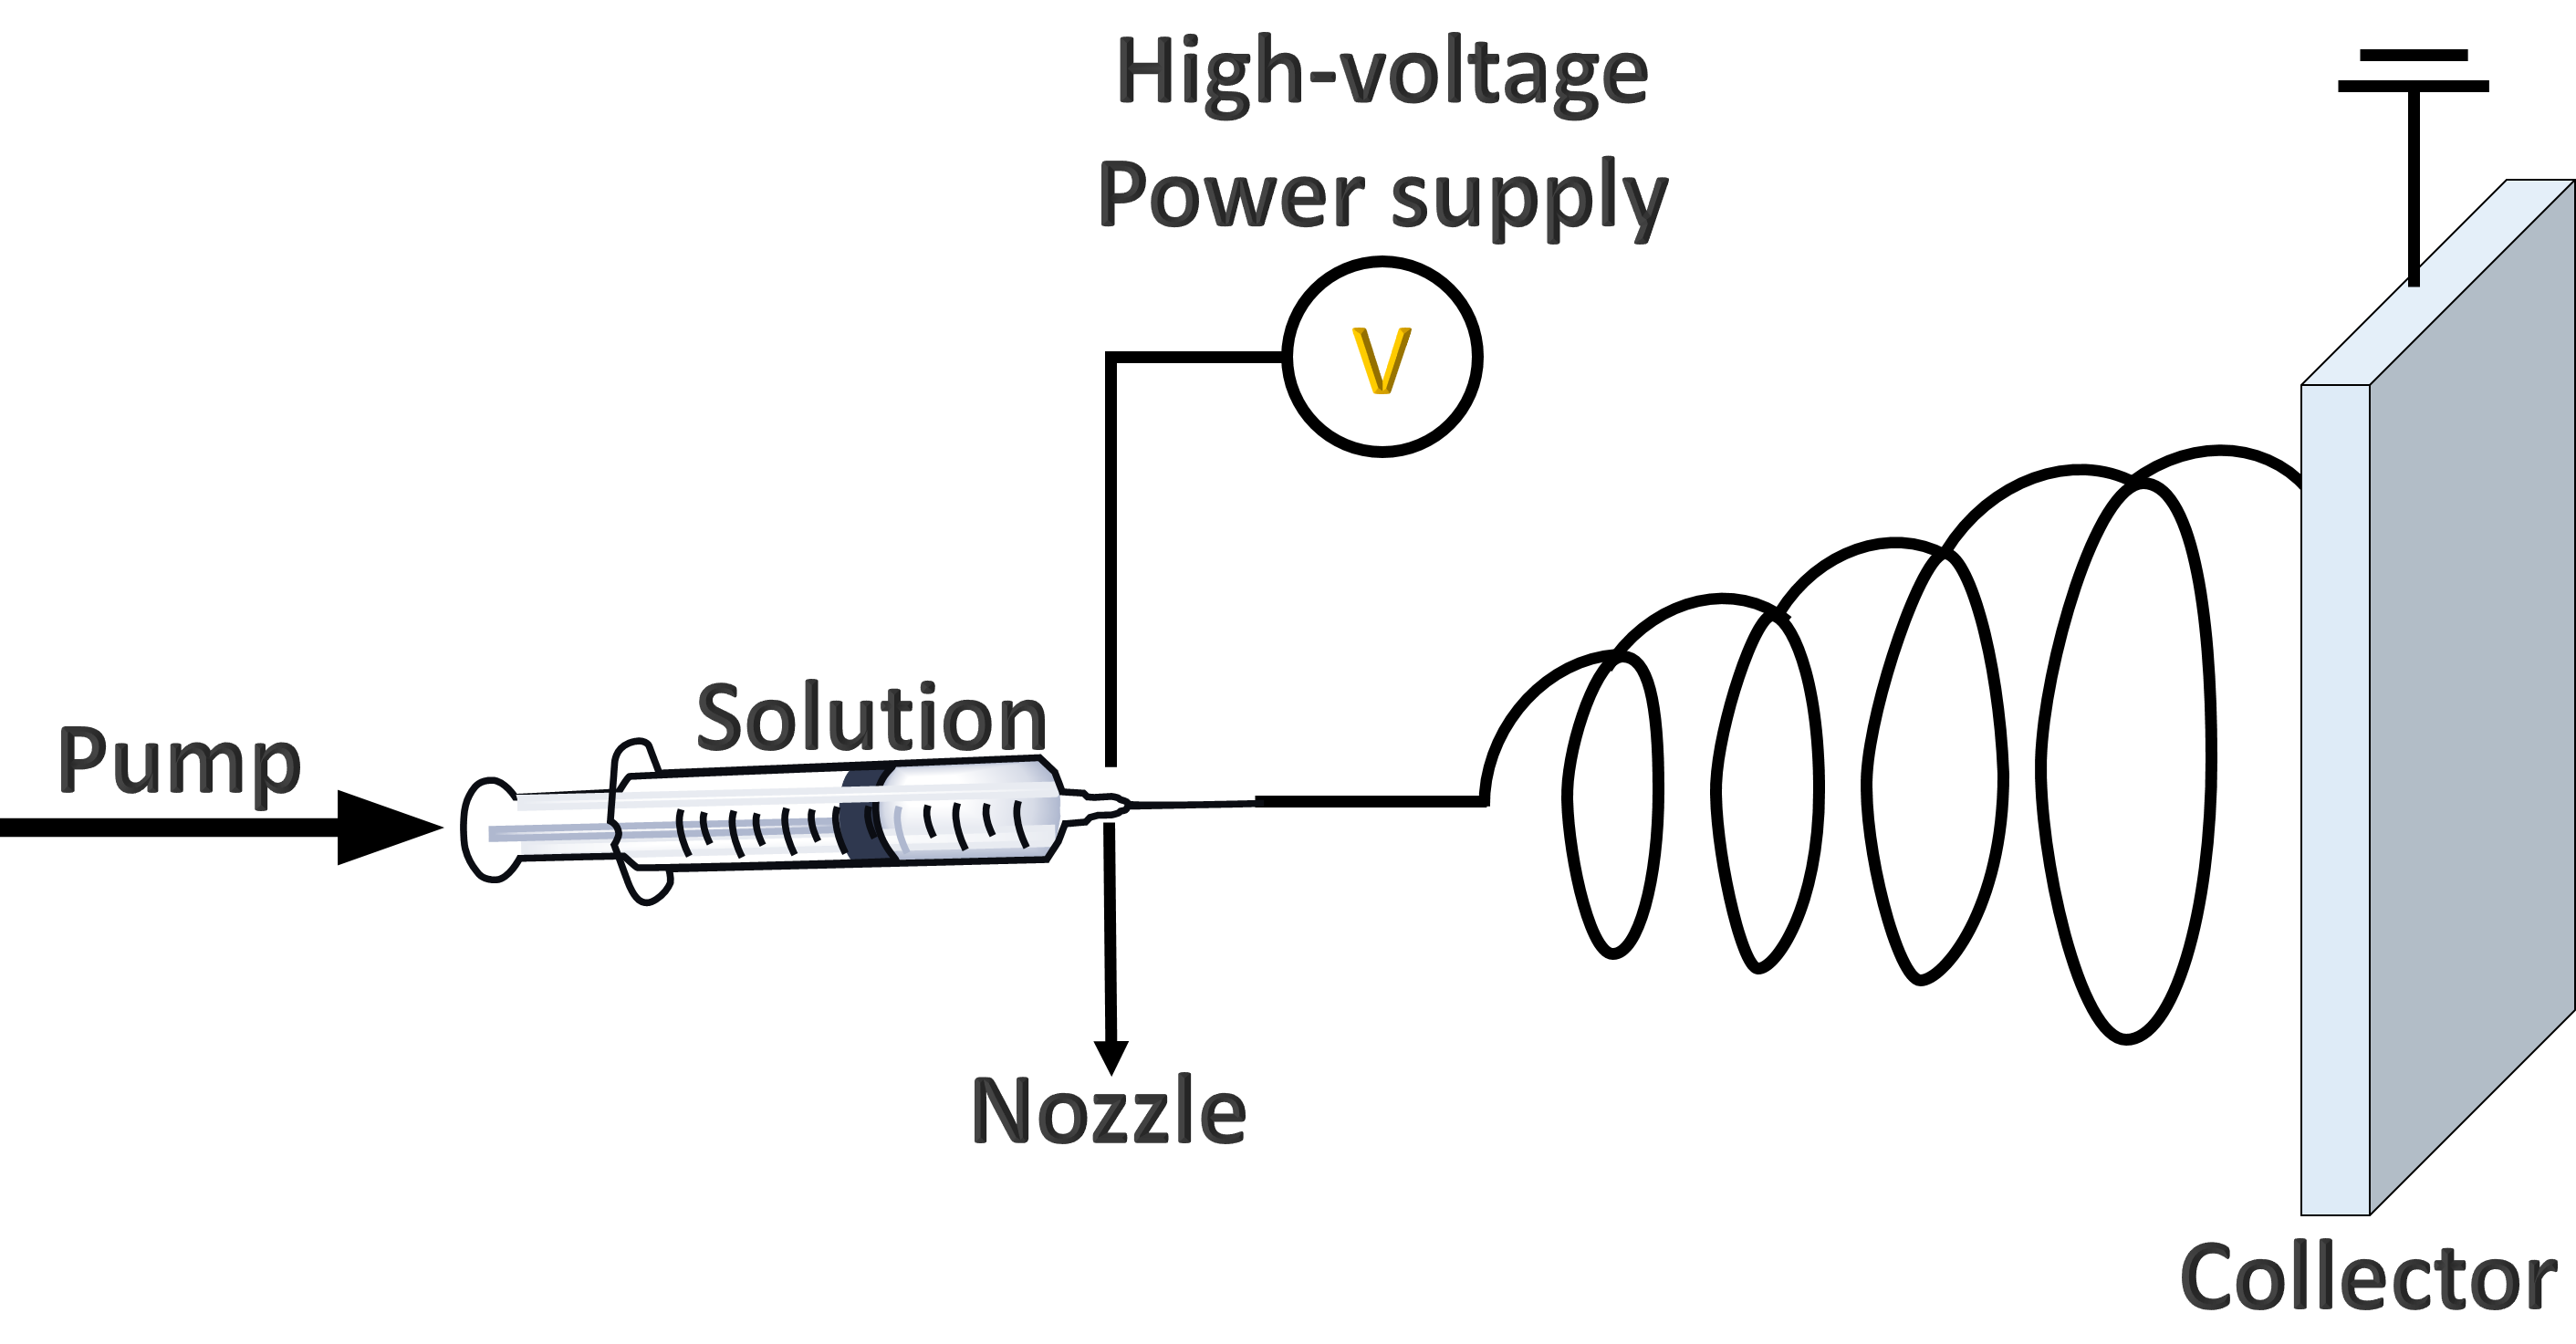
\includegraphics[width=\textwidth]{Figures/chap6fig/electrospinning}
\caption{A schematic illustration of an electrospinning setup.}
\label{Figures/chap6fig:electrospinning}
\end{figure}

\subsection{Experimental methods}
Electrospun \ce{SnO2} fibers were obtained from University of Montpellier, France and was used as received. \\
\textbf{Electrospinning} is an electrostatic fiber fabrication technique. It uses electrical forces to produce polymer fibers with diameters ranging from 2nm to a few $\mu$m. The techniques utilizes solution of both natural and synthetic polymers \cite{bhardwaj_electrospinning_2010}. The fibers obtained via electrospinning have smaller pores and a higher surface area than regular fibers produced by standard mechanical fiber-spinning technology \cite{huang_review_2003}. An electrospinning setup is illustrated in Figure \ref{Figures/chap6fig:electrospinning}. The topography and orientation of the fibers can be controlled by modifying parameters such as voltage, pump speed or nozzle thickness in the electrospinning setup.


\subsection{Results and discussion}
To evaluate the electrochemical properties, the Al/\ce{SnO2} cell was charged and discharged at constant current between 0.2-2.35 V at current rates ranging from 50-1500 mA g$^{-1}$. Figure \ref{Figures/chap6fig:SnO2newCDC} displays the voltage vs. specific capacity plot of the AIB. The curves demonstrate a well defined discharge plateau at $\sim$ 0.55 V. In the first cycle, the battery achieved a capacity of 105 mAh g$^{-1}$, which decreased to 50 mAh g$^{-1}$ after 120 cycles. CE of the cell decreased with every cycle and reduced to <60\% after 500 cycles. The discharge capacity decreased after every cycle and reached a value of $\sim$20 mAh g$^{-1}$ after 500 cycles, it might be possible that electrospun fibers suffered repeated expansion and contraction during the cycles, which caused cathode pulverisation. As a result \ce{SnO2} failed to deliver a stable performance. Distinct voltage plateaus indicate reversible redox processes taking place during charge and discharge. To confirm the redox activity, cyclic voltammetry was performed and the resultant scans are displayed in Figure \ref{Figures/chap6fig:Sno2CV}. The CV exhibits a reduction peak at 0.45 V and an oxidation peak at 0.55 V, which match perfectly with the discharging voltage plateau observed at 0.47 V and charging voltage plateau at 0.55 V respectively.    

 \begin{figure}[th!]
  \centering
  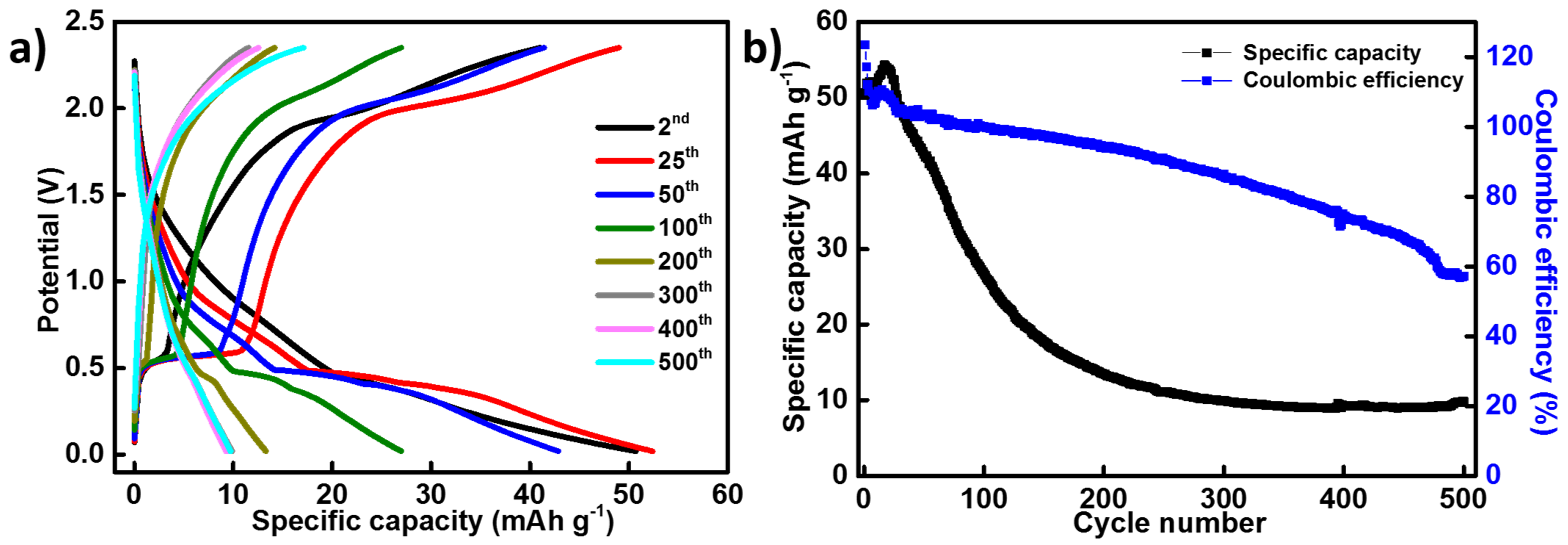
\includegraphics[width=\textwidth]{Figures/chap6fig/SnO2newCDC}
    \caption{a) Galvanostatic charge and discharge curve of an Al/\ce{SnO2} cell at the current rate of 40 mA g$^{-1}$. b) Long-term stability test of the cell.}
  \label{Figures/chap6fig:SnO2newCDC}
\end{figure}

\begin{figure}[th!]
\centering
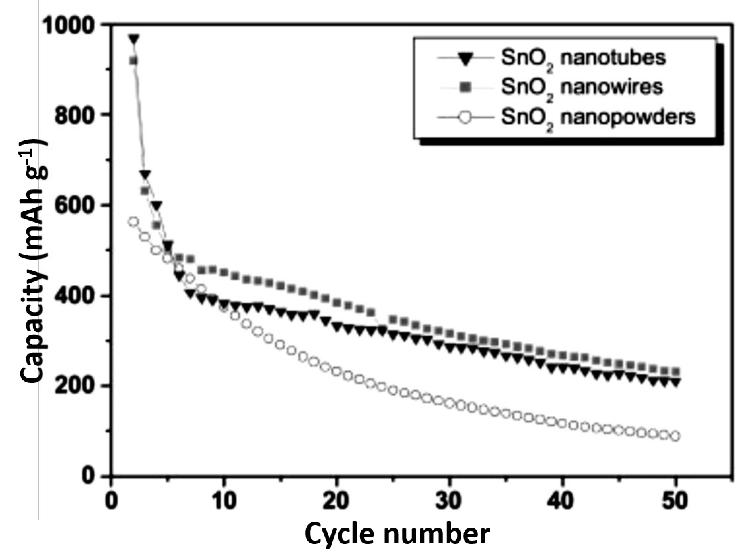
\includegraphics[width=0.75\textwidth]{Figures/chap6fig/sno2pap.pdf}
\caption{The cyclic performance of \ce{SnO2} nanomaterials in lithium-ion batteries up to the fiftieth cycle at a current density of 100 mA g$^{-1}$. Capacity of the materials decreases with every cycle due to expansion of \ce{SnO2}, which leads to cathode pulverisation and capacity fading \cite{park_effect_2008}.}
\label{Figures/chap6fig:sno2pap}
\end{figure}

However, the X-ray diffraction patterns in Figure \ref{Figures/chap6fig:SnO2XRD} look alike after charge and discharge except a shoulder that develops in the charged and discharged cathodes at 2$\theta$ value of 22$^{\circ}$. Sharp Bragg peaks correspond to the crystalline phase and the broad bump under the peaks at 22$^{\circ}$ and  34$^{\circ}$ observed in the charged cathode corresponds to the amorphous state of the same material. Since the X-rays were scattered in many directions leading to a large bump distributed in a wide range. Furthermore, the peak at  51$^{\circ}$ splits after charge. The peak splitting might suggest formation of another crystal structure or presence of secondary phase that was formed during charge. SEM images in Figure \ref{Figures/chap6fig:SnO2SEM} display the cathode morphology before and after cycles where a few fibers show signs of damage after charge/discharge in Figure \ref{Figures/chap6fig:SnO2SEM}c. 

 \begin{figure}[th!]
  \centering
  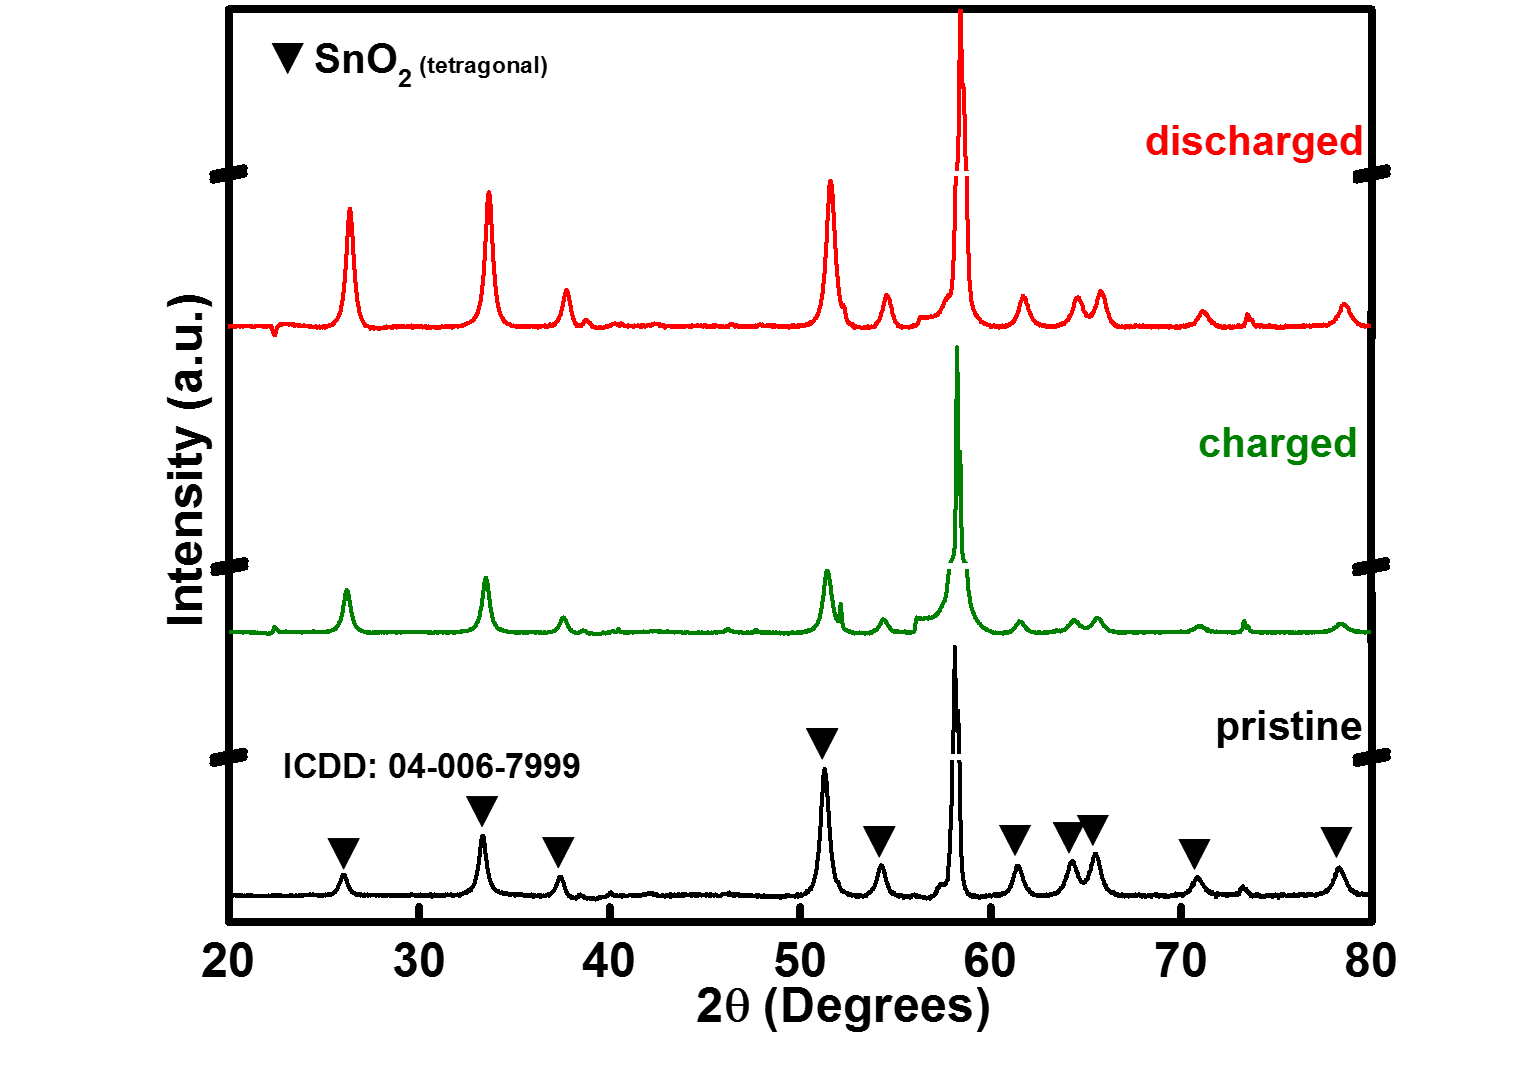
\includegraphics[width=0.8\textwidth]{Figures/chap6fig/SnO2XRD}
    \caption{\textit{Ex-situ} X-ray diffraction patterns of \ce{SnO2} cathode in a pristine (black), charged (green) and discharged (red) state.}
  \label{Figures/chap6fig:SnO2XRD}
\end{figure}

 \begin{figure}[th!]
  \centering
  
\includegraphics[width=0.8\textwidth]{Figures/chap6fig/Sno2CV}
    \caption{\textit{Ex-situ} X-ray diffraction patterns of \ce{SnO2} cathode in a pristine (black), charged (green) and discharged (red) state.}
  \label{Figures/chap6fig:Sno2CV}
\end{figure}

Further analysis such as \textit{in-situ} XRD or an \textit{ex-situ} XPS analysis of the charged and discharged cathodes is needed to investigate whether \ce{SnO2} follows a similar type of charge storage in AIBs as it does in LIBs. It would be interesting to find out whether new complexes are being formed after \ce{AlCl4-} anions interact with \ce{SnO2} during charge/discharge cycles. 


\section{Molybdenum trioxide}

\subsection{Introduction}

 \begin{figure}[th!]
  \centering
  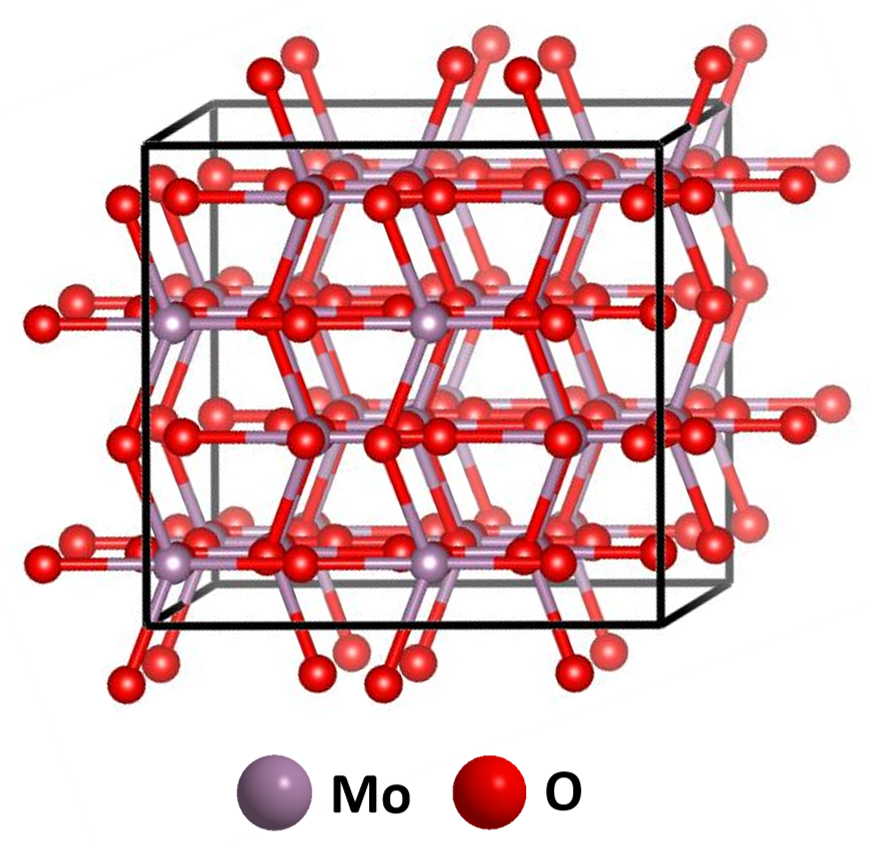
\includegraphics[width=\textwidth]{Figures/chap6fig/MoO3crys}
    \caption{Crystal structure of \ce{MoO3}.}
  \label{Figures/chap6fig:MoO3crys}
\end{figure}

Molybdenum trioxide, \ce{MoO3} is an intermediate formed during production of molybdenum metal. It has a layered orthorhombic arrangement with a space group of Pnma, and contains four formula units of \ce{MoO3} per unit cell. The single sheet adopts a bilayer structure with both sides of the surface terminated with oxygen atoms. The crystal structure of \ce{MoO3} is illustrated in Figure \ref{Figures/chap6fig:MoO3crys}. Due to its layered structure, \ce{MoO3} has been popularly used as an electrode material in LIBs \cite{wu_mixed_2017,li_vapor-transportation_2006,tsumura_lithium_1997}. The intercalation of \ce{Li+} ions and the resulting redox reactions resulted in capacities ranging from 200-400 mAh g$^{-1}$ \cite{tsumura_lithium_1997,chen_fast_2010,zhou_-moo3_2010}. As one of the earliest studied host materials for \ce{Li+} insertion, $\alpha$ \ce{MoO3} can accommodate $\sim$ 1.5 lithium per Mo atom. Lithiated \ce{MoO3} (\ce{LixMoO3}) displayed good electronic conductivity and high \ce{Li+} mobility. It has been reported that the \ce{Li+} ions insert not only into the interlayer spacing between the \ce{MoO6} octahedron layers but also into the \ce{MoO6} intralayers \cite{li_vapor-transportation_2006,chen_fast_2010}. However, high concentrations of unsolvated \ce{Li+} in the host lattice sometimes causes irreversible structural changes resulting in poor cell performance \cite{tao_moo3_2011,li_theoretical_2014}.\\
The reaction that takes place inside a LIB during discharge is given below \cite{li_vapor-transportation_2006}. 

\begin{equation}
    \ce{xLi+ + MoO3 + xe- -> Li_{x}MoO3} 
\end{equation}

The given reaction is reversed during charge.

\ce{MoO3} has also been used as a cathode material in aqueous AIBs \cite{joseph_hexagonal_2019, shakir_structural_2010, lahan_al3+_2019, lahan_active_2018}. Lahan and Das \textit{et al.} reported that intercalation of \ce{Al^{3+}} cations was possible in orthorhombic \ce{MoO3}. However the performance was dependent on the electrolyte composition. They demonstrated that \ce{MoO3} stored more \ce{Al3+} ions when \ce{AlCl3} was used instead of \ce{Al2(SO4)_3} and Al\ce{(NO3)_3}. It also minimized the cell polarization and improved the long-term stability of the cell. \ce{MoO3} cell achieved a specific capacity of 680 mAh g$^{-1}$ (highest reported value for any aqueous AIB) after its first discharge cycle. \\ 
Since \ce{MoO3} was never tested before as a cathode in non-aqueous AIBs, it was used as an active material for this project. However, in 2018 (after the preliminary tests for this PhD thesis were completed), Nacimiento \textit{et al.} used layered-type $\alpha$-\ce{MoO3} as a cathode in non-aqueous AIBs using \ce{AlCl3}:EMIC in the ratio of 1.1:1.0 (slightly acidic melt) as the electrolyte. The maximum capacity achieved was 100 mAh g$^{-1}$, which decreased to 85 mAh g$^{-1}$ after 7 cycles. In addition, a rapid capacity decay was observed in Figure \ref{Figures/chap6fig:moo3pap}. After 11 cycles, the capacity decreased to 40 mAh $^{-1}$ at a low current rate of 3 mA g$^{-1}$. 

\begin{figure}[th!]
\centering
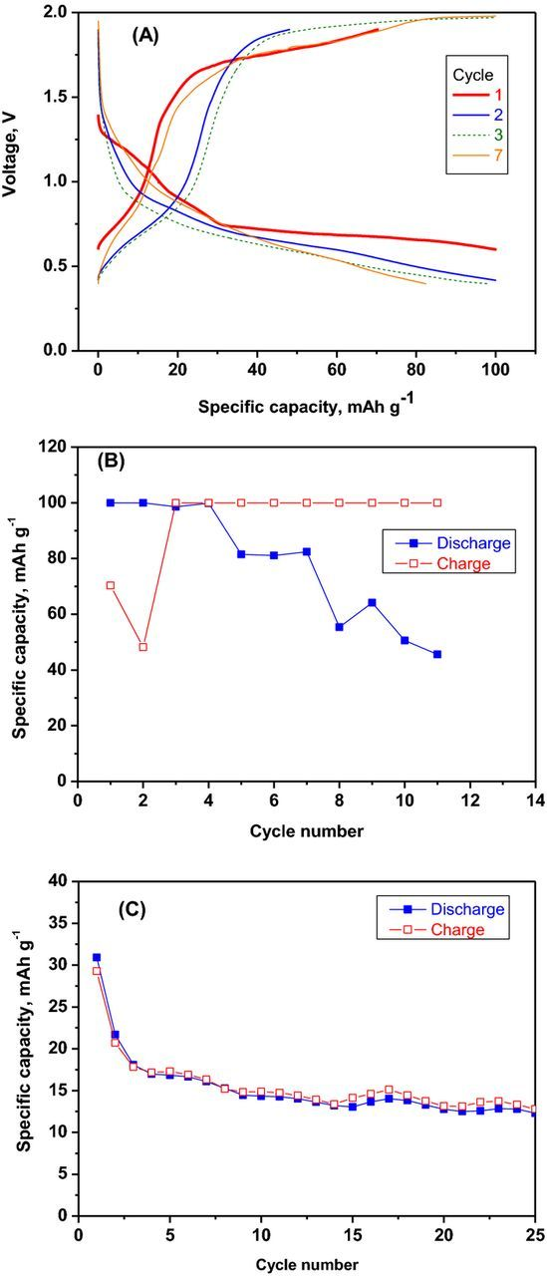
\includegraphics[width=0.5\textwidth]{Figures/chap6fig/moo3pap}
\caption{Galvanostatic experiments for MoO3 in aluminum cell. A) Voltage-capacity curves and, B) corresponding capacity as a function of cycle number at current density 3 mA g$^{-1}$, and C) capacity as a function of cycle number at 10 mA g$^{-1}$ for 0.1-2.1 V of voltage limits \cite{nacimiento_exploring_2018}}
\label{Figures/chap6fig:moo3pap}
\end{figure}

\subsection{Experimental methods}
Molybdenum trioxide (\ce{MoO3} ACS reagent, $\geq$99.5\% was purchased from Sigma-Aldrich and used as received.

\subsection{Results and discussion}
At a high current rate of 1500 mA g$^{-1}$ (Figure \ref{Figures/chap6fig:MoO3cdcce}a),\ce{MoO3} achieved the highest capacity of $\sim$80 mAh g$^{-1}$ with CE>100\%. After 120 cycles, the cell managed to retain 75\% of its original capacity. Voltage bends were observed during charge at 2.0 and 1.7 V for the first 100 cycles and a plateau was observed during discharge at 1.4 V. Discharge capacities at various current densities ranging from 50 mA g$^{-1}$ to 1500 mA g$^{-1}$ have been shown in Figure \ref{Figures/chap6fig:MoO3cdcce}. This cell performed better than Nacimiento's cell displaying higher discharge capacities and displayed better capacity retention during discharge.  

\begin{figure}[th!]
\centering
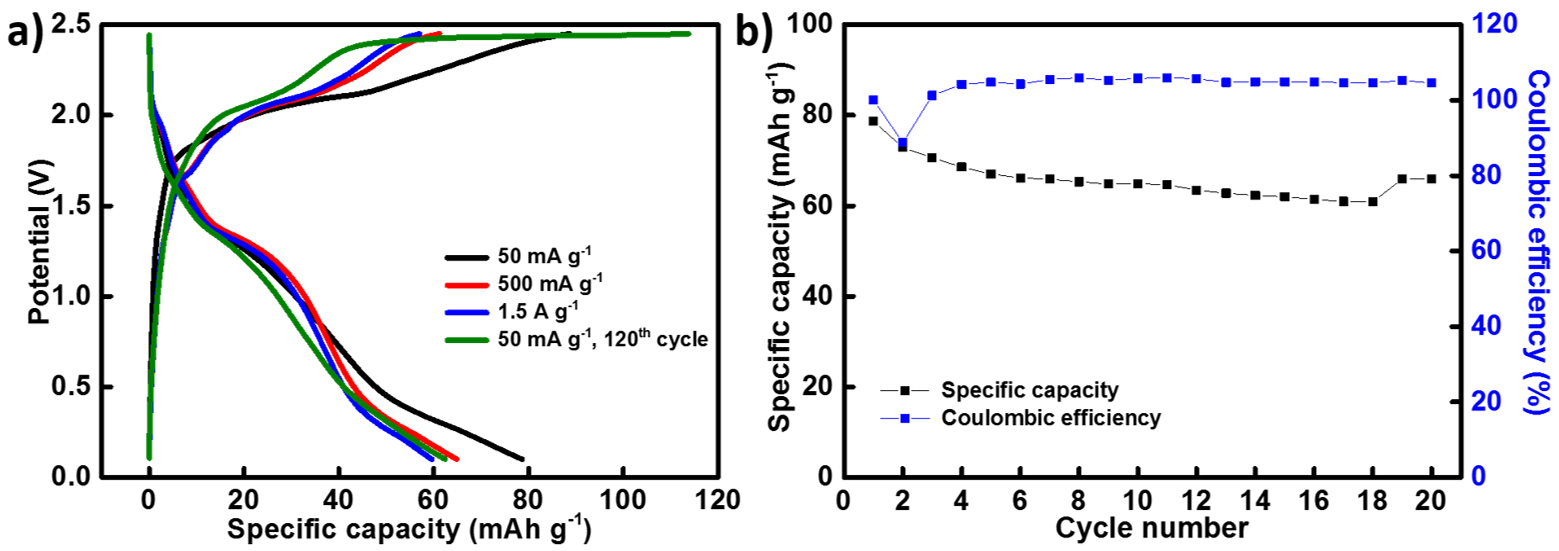
\includegraphics[width=\textwidth]{Figures/chap6fig/MoO3cdcce}
\caption{Charge/discharge cycles of an Al/\ce{MoO3} cell at various current rates.}
\label{Figures/chap6fig:MoO3cdcce}
\end{figure}

\subsection{Summary and conclusions}
The electrochemical data suggests fast intercalation-based redox reactions similar to LIBs. With an energy density of $\sim$85 Wh kg$^{-1}$, this material shows a lot of potential for high-performing AIBs. 


\section{Graphitic Carbon Nitride}

\subsection{Introduction}
Graphitic carbon nitride or g-\ce{C3N4} is a carbon-based material that was first synthesised in 2012. The material is highly stable under physiological conditions and displays semiconductive properties. The crystal structure can be regarded as N-substituted graphite framework consisting of $\pi$-conjugated graphitic planes formed via sp$^2$ hybridisation of C and N atoms. The inter-layer distance between two stacks is 3.26\AA, and is 2\% more densely packed than crystalline graphite \cite{zheng_graphitic_2012}. Due to N-atom substitution, the binding between two layers is strengthened, which decreases its inter-layer distance. g-\ce{C3N4} is a low-cost metal free material with a high surface area \cite{zheng_graphitic_2012}. Since the structure of g-\ce{C3N4} is analogous to graphite, it has been used for electrochemical energy storage applications. \\*
g-\ce{C3N4} has been used as a battery electrode material in LIBs, Li-\ce{O2}, Li-S, Zn-air, vanadium redox flow batteries and SIBs. The presence of \enquote{pyridinic} N in g-\ce{C3N4} favors high \ce{Li+} intake and prohibits irreversible reactions. Therefore, nitrogen content and its type, highly influence the performance of g-\ce{C3N4} in LIBs \cite{shah_highly_2017}. \\*
Vanadium redox flow batteries on the other hand, have also used g-\ce{C3N4} as a catalyst. A typical vanadium redox flow battery consists of two electrolyte tanks with \ce{VO2+}/\ce{VO^{2+}} and \ce{V3+}/\ce{V2+} redox couples, two pumps and a battery cell. The electrochemical reactions take place at the electrode. For this reason, highly efficient catalysts are needed. Huang \ce{et al.} modified carbon felt (usually used as a catalyst in flow batteries) with g-\ce{C3N4} for catalyzing the redox reactions. This increased the energy efficiency (EE) of the cells to 87\%. In addition, Nafion membranes were replaced by g-\ce{C3N4} hybrids, such as sulfonated poly(ether ether ketone) SPEEK/g-\ce{C3N4} and oxidised g-\ce{C3N4} (OCN) ion membranes \cite{niu_novel_2017, wang_novel_2017}. An ion membrane separates the ion-pairs in the flow battery and accelerates the proton flow during charge/ discharge cycles. The g-\ce{C3N4} modified membranes not only improved the EE of the flow batteries but also increased its efficiency (CE: 97\% and EE: 83.6\%) when compared to Nafion (CE: 90\% and EE: 73.8\%). A good structure stability against strong oxidizing and acidic condition was reported. The acid-base pairs formed between -\ce{NH2} groups of g-\ce{C3N4} and sulfonic acid groups of SPEEK enhanced the vanadium ion permeability and its selectivity, and also improved the proton transport channel \cite{wang_novel_2017}. SPEEK/OCN membranes due to their high surface area and intrinsic stability of OCN contributed to decrease the vanadium ion permeability. The functional groups of OCN helped in improving the proton conductivity and improved the battery's performance. Due to all of the above-mentioned properties such as high surface area and structural stability, g-\ce{C3N4} was tested as a cathode material for non-aqueous AIBs. It was speculated that the chloroaluminate ions would undergo a similar intercalation-type process that would be supported by the graphitic framework present in g-\ce{C3N4}.

\subsection{Experimental methods}
g-\ce{C3N4} that was synthesised using urea and was obtained from the University of Auckland. The material was used as received for making the slurry. 

\subsection{Results and discussion}
Figure \ref{Figures/chap6fig:CNUcdccv}a and b shows the charge/discharge curves and CV scan of g-\ce{C3N4} cell. The discharge capacity decreased from 160 mAh g$^{-1}$ to $\sim$100 mAh g$^{-1}$ after 120 cycles at the current rate of 50 mA g$^{-1}$. Figure \ref{Figures/chap6fig:CNUcdccv}a shows the discharge capacities at current densities ranging from 50 mA g$^{-1}$ to 1500 mA g$^{-1}$. The cell managed to achieve a capacity of 95 mAh g$^{-1}$ at 500 mA g$^{-1}$. A distinct charging plateau at 2.1 V and a slight bend during discharge at 0.6 V suggests the presence of reversible redox reactions. However, the capacity decreased to almost zero at 1500 mA g$^{-1}$, which implies that the current was too high and the cell was not allowed to complete its reaction. 

\begin{figure}[th!]
\centering
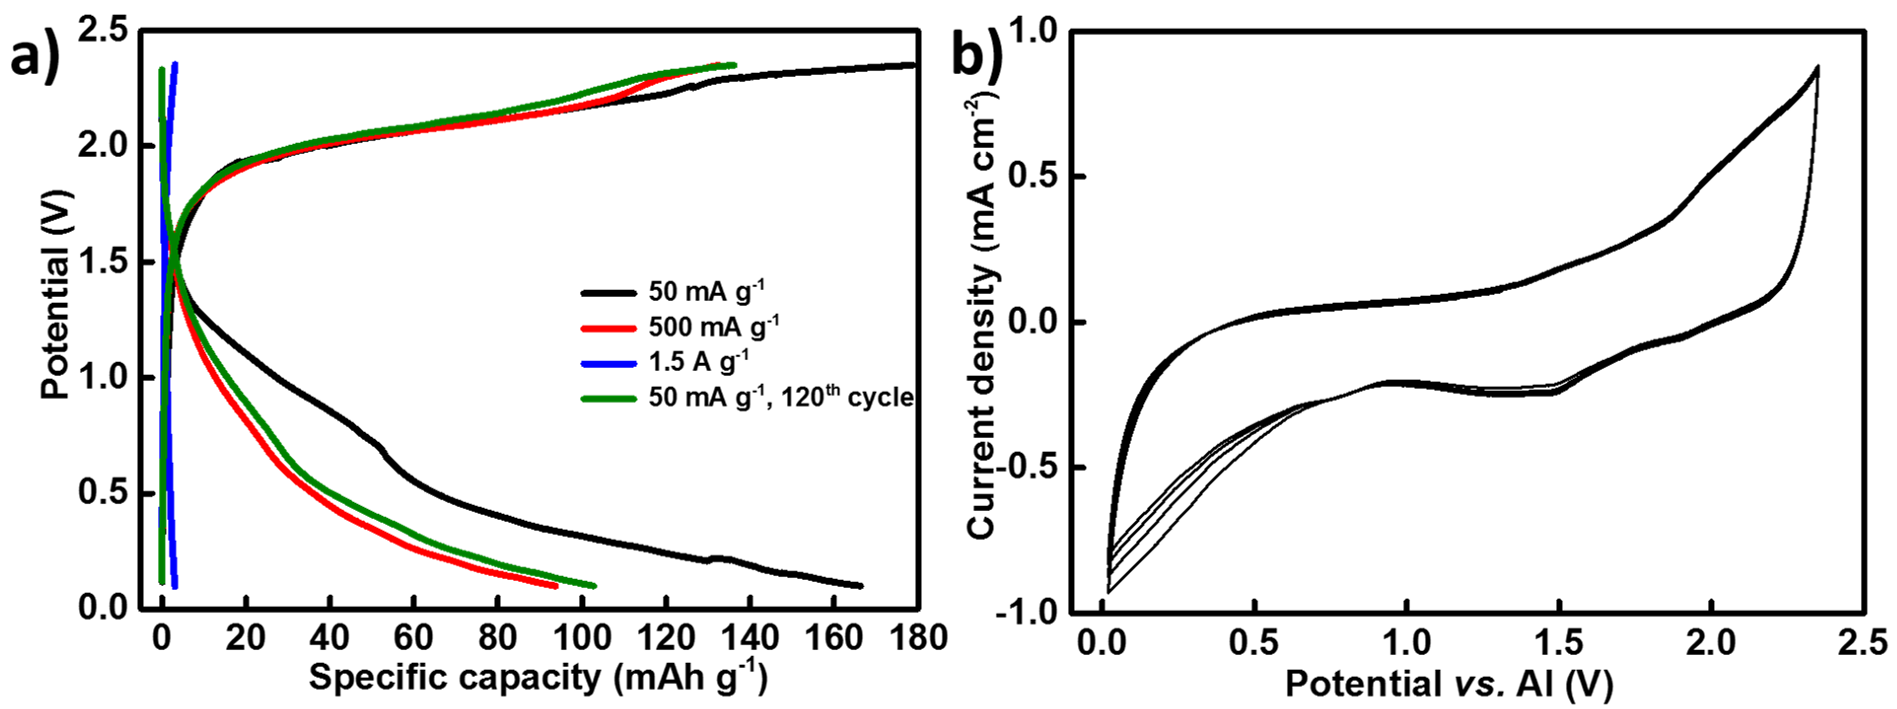
\includegraphics[width=\textwidth]{Figures/chap6fig/CNUcdccv}
\caption{a) Charge/discharge cycles of an Al/\ce{MoO3} cell at various current rates. The cell managed to retain 67\% of its original capacity after 120 cycles. b) Cyclic voltammogram of an Al/g-\ce{C3N4} cell; a reduction peak at 1.6 V was observed, which does not correspond to any of the voltage bends or plateaus observed in the charge/ discharge curves. }
\label{Figures/chap6fig:CNUcdccv}
\end{figure}

The storage performance of g-\ce{C3N4} in other battery systems was largely affected due to its large contact resistance and low band-gap \cite{shah_highly_2017}. Considerable efforts were made to improve its performance. Despite the fact that g-\ce{C3N4} has a more open structure than graphite, which should improve its \ce{Li+} intake and exchange capability, Luo \cite{luo_graphitic_2019} \textit{et al.} showed that the LIB using g-\ce{C3N4} anode displayed a capacity of 134.9 mAh g$^{-1}$ and an irreversible capacity loss of >98\% after 7 cycles. Veith and Hankel \textit{et al.} reported that reactions of lithium with g-\ce{C3N4} was responsible for the irreversible capacity loss \cite{veith_electrochemical_2013, hankel_lithium_2015}. Furthermore, replacement of C atoms with N atoms in the benzene ring was also proven to be responsible for its poor conductivity. These reasons might be valid for an AIB system as well since the material failed to retain its capacity. Nevertheless, there is still scope for improvement as new functional groups can be added to g-\ce{C3N4} that might improve its charge-storing capacity. The basic structural units used to build g-\ce{C3N4} are the triazine (\ce{C3N4}) and the tri-\textit{s}-triazine/ heptazine (\ce{C6N7}) ring. The two structures possess different energetic stabilities because of their different electronic environments of the N atoms and the size of the nitride pores. Density functional theory (DFT) calculations demonstrated that the tri-\textit{s}-triazine based g-\ce{C3N4} was more stable and energetically favored. Hence, tri-\textit{s}-triazine is broadly recognized as the basic unit for the formation of the 2D sheets of g-\ce{C3N4}. Hence it is important to determine which one of the two rings formed the g-\ce{C3N4} structure. If it was triazine, modifications can be made so that tri-\textit{s}-triazine rings are formed that increase the charge-storing capacity of the cell. 

\begin{figure}[th!]
\centering
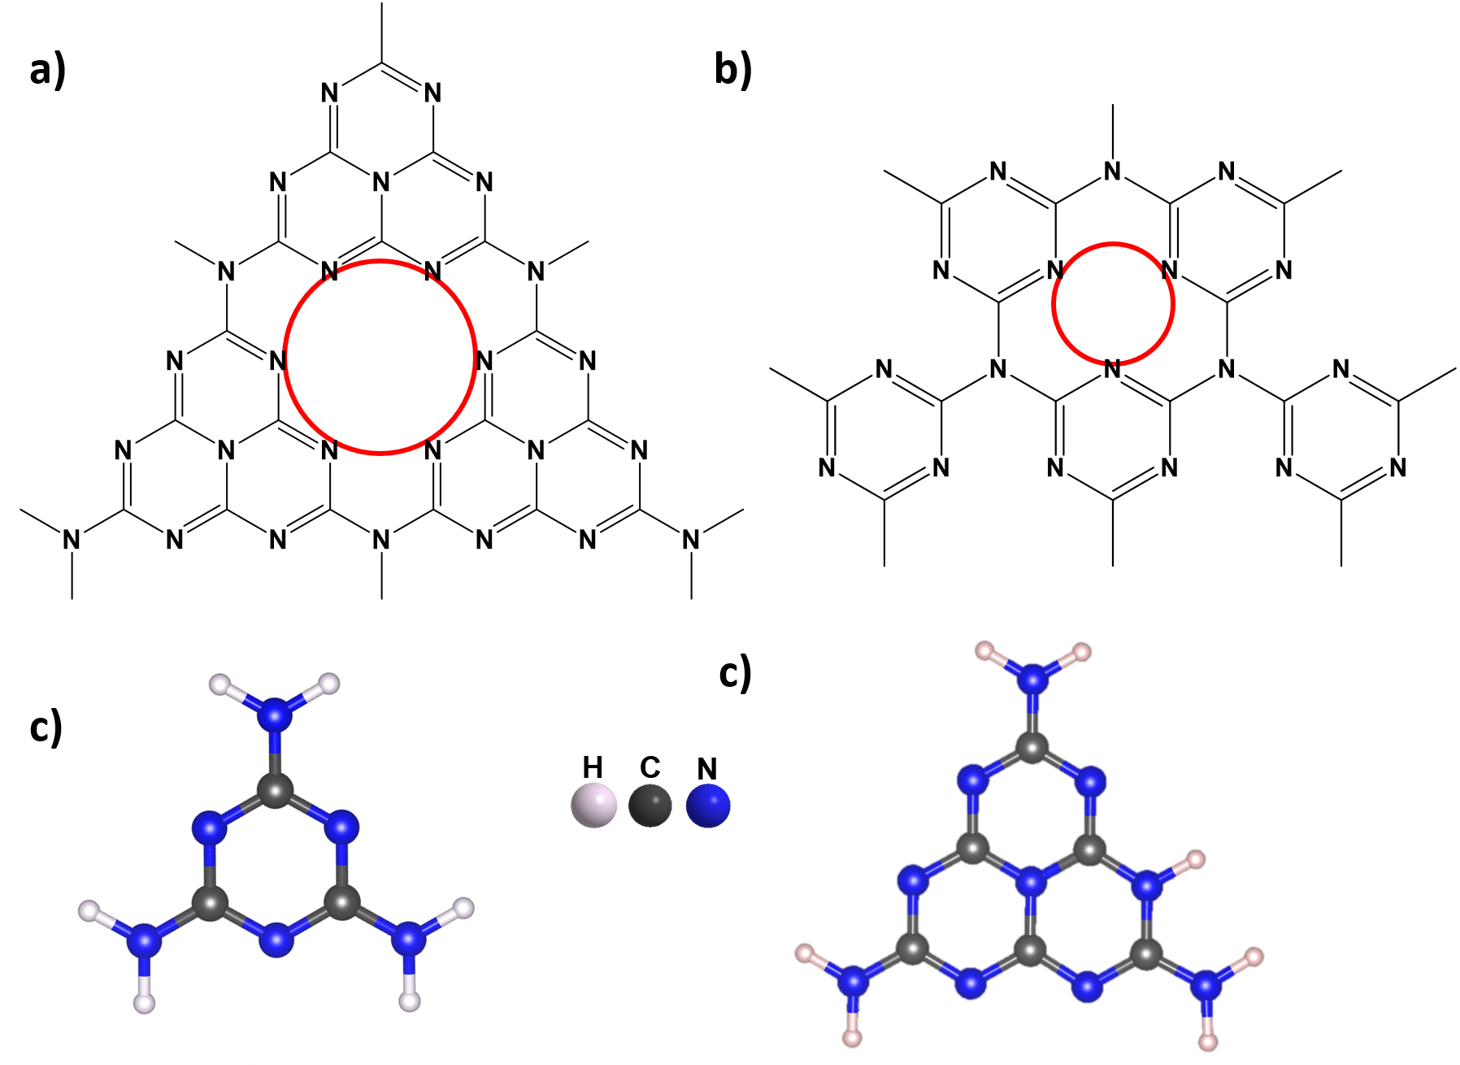
\includegraphics[width=\textwidth]{Figures/chap6fig/c3n4}
\caption{Structural motifs for graphitic-carbon nitride (g-\ce{c3N4}) molecules: s) fully condensed polyheptazine (tri-\textit{s}-triazine) \ce{C3N4} structure, and b) fully condensed triazine based \ce{C3N4} structure.}
\label{Figures/chap6fig:c3n4}
\end{figure}

\section{Prussian blue}

\subsection{Introduction}

 \begin{figure}[th!]
  \centering
  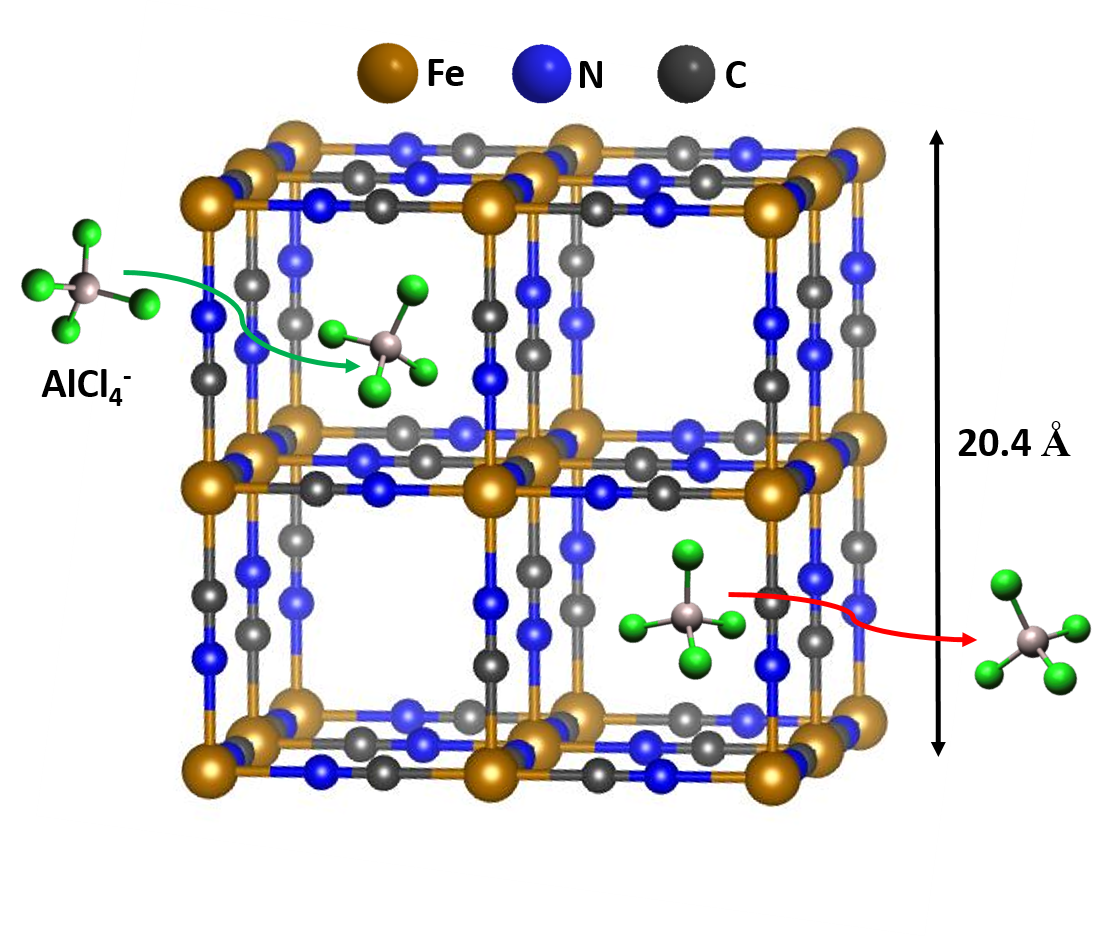
\includegraphics[width=\textwidth]{Figures/chap6fig/pbcrys}
    \caption{Crystal structure of Prussian blue. The voids present in the framework (20.4\AA) are spacious enough to allow the chloroaluminate ions (5.36\AA) to move in and out of it during charge and discharge. }
  \label{Figures/chap6fig:pbcrys}
\end{figure}

Prussian blue belongs to the family of metal-organic framework, also known as MOF. A MOF is a hybrid crystalline porous material. It consists of a regular arrangement of positively charged metal ions and surrounded by organic molecules. A repeating cage-like structure is formed when metal cations form nodes that binds with an organic molecule's linker. MOFs have a large surface area (as high as 700 m$^{2}$g $^{-1}$) due to their hollow structure. Figure \ref{Figures/chap6fig:pbcrys} displays the crystal structure of Prussian Blue. The structural uniformity and and the flexibility in their network topology, makes MOF an ideal battery material. Its open framework allow insertion of ions in the sub-cages. The structure has a number of redox sites present as each molecular formula contains two redox centres \ce{M+2}/\ce{M3+}, where M is any transition metal (Fe, Co, Ni, Mn, Cu, Zn). It reaches 2\ce{e-} redox capacity after reversibly intercalating 2 monovalent alkali ions per molecular unit. Presence of large lattice interstices and ionic channels renders a high specific capacity. The ability to tune MOFs along with its structural design, makes it different from the conventional porous materials. Due to their high surface area and and tailored pore-size, MOFs have been utilised as electrode materials in electric double layer capacitors or EDLCs, LIBs and SIBs. A Co-Zn MOF was designed by Diaz \textit{et al.} and it showed a typical EDLC behaviour in a non-aqueous electrolyte \cite{diaz_co8-mof-5_2012}. However, the specific capacitance for Co-Zn MOF was low. It was observed that cobalt-based MOF derived from Co\ce{(NO3)_2}, displayed pseudocapacitance behaviour (presence of redox couples) instead of an EDLC behaviour with an improved specific capacitance. Lee \ce{et al.} observed a relationship between the pore size of MOFs and their performance in supercapacitors. After several attempts, it was determined that inclusion of conducting species within the MOF framework could solve the problem of low capacitance by providing an efficient electron pathway. Furthermore, MOFs with tailored channels or pores would allow faster diffusion of active ions during charge/ discharge cycles. The electrolyte also plays an important role in achieving high-performing supercapacitors. \\*
Recently, MOFs have been investigated as anode materials in LIBs \cite{li_shape-controlled_2006,han_synthesis_2012,zhao_metalorganic_2015}. To be used as anodes, the porous structure of MOFs allows reversible intercalation of \ce{Li+} ions during charge/discharge cycles. MOF-177 was the first MOF that was used as an anode material in LIBs \cite{}. The material underwent a conversion reaction inside the cell that destroyed its structure and consequently resulted in a poor cycling performance.  Zhang \textit{et al.} investigated Prussian blue nanoparticles as anodes \cite{nie_prussian_2014}. The open-framework structure allowed rapid intercalation/ de-intercalation of \ce{Li+} ions. The cell achieved a reversible capacity of 300 mAh g$^{-1}$ and superior rate capability. Yagi and his group studied the lithiation mechanism in Prussian blue and its analogues (PBAs) \cite{yagi_eqcm_2014}. They reported that the redox reaction of PB might also proceed with the electrochemical adsorption/ desorption of \ce{PF6-} ions, which are the counter ions in the electrolyte. MOFs have also been used as templates for preparing nanostructured metal oxides and and carbon materials. A few other MOFs used in LIBs as anode materials have been listed in Table \ref{tableMOF}. \ce{Li+} storage in a typical LIB takes place via the following mechanisms: \\

\textbf{Conversion reaction}- metal ions present in the MOF get replaced by \ce{Li+} ions \\
\textbf{Intercalation reaction}- \ce{Li+} ions get stored in the MOF's cage-like structure and keeps the structure intact \cite{wang_metalorganic_2016}. \\

MOFs have shown to have many applications in electrochemical energy storage. They can be used both in supercapacitors and in batteries. Based on the multiple valence of metal ions, open framework and ligands with functionalities, novel electrode materials can be designed from MOFs and used in AIBs. For this reason, Prussian blue, a popular MOF, was tested as a cathode material in this project. 

\vspace{0.5cm}
\begin{table}
\centering
\caption{Summary of performances of MOFs used as anode and cathode materials in various energy storage devices.} \label{tableMOF}
\begin{tabular}{ |p{1cm}|p{3.5cm}|p{2.2cm}|p{1.2cm}|p{1.5cm}|}
 \hline 
\textbf{Ref.} & \textbf{MOFs} & \textbf{Capacity (mAhg$^{-1}$)/ Capacitance (Fg$^{-1}$)} & \textbf{Voltage (V)} & \textbf{Surface area (m$^{2}$g$^{-1}$)} \\ 
\hline
\cite{li_shape-controlled_2006} & {MOF 177} & 425 & 0.1-1.6 & -\\
\cite{han_synthesis_2012} & Li/Ni-NTC & 1084 & 0.01-3 & -\\
\cite{zhao_metalorganic_2015} & Asp-Cu nanofibers & 1255 & 0.01-3 & -\\
\cite{wu_mof-templated_2013} & CuO & 1208 & 0.05-3 & -\\
\cite{huang_metal-organic_2014} & \ce{Fe2O3}/\ce{NiCo2O4} & 1311 & 0.01-3 & -\\
\cite{nagarathinam_redox-active_2012} & \ce{K2.5VO2}\ce{HPO4}\ce{C2O4} & 62 & 2.5-4.6 & -\\
\cite{zhang_monitoring_2014} & Cu(2,7-AQDC) & 147 & 1.7-4 & -\\
\cite{liu_metalorganic_2010} & NPC650 & 222 & - & 1521\\
\cite{hu_porous_2010} & MC-A & 208 & - & 1674\\
\cite{tang_thermal_2015} & NC/GC & 270 & - & 1276\\
\cite{chen_high-performance_2013} & N-PC & 219 & - & 484\\
\cite{banerjee_mof-derived_2014} & MOF-DC & 149 & - & 2714\\
\hline
\end{tabular}
\end{table}

\subsection{Results and discussion}
The first charge–discharge curve exhibited distinct voltage bends and plateaus at 1.8, 1.2 V and 0.6 V with a capacity reaching $\sim$140 mAh g$^{-1}$ after first 20 cycles. To investigate the rate capabilities of the battery, the cell was charged and discharged at various current densities (Figure \ref{Figures/chap6fig:pbcdccecv}a) ranging from 50-1500 mA g$^{-1}$. The specific capacities and CEs over 180 cycles at different current rates are shown in Figure \ref{Figures/chap6fig:pbcdccecv}b. Discharge capacity after the first cycle is 140 mAh g$^{-1}$, and it exhibits multiple discharge voltage plateaus. With an increase in current density, the capacity of the battery gradually decreased to 5 mAh g$^{-1}$. 

 \begin{figure}[tbh!]
  \centering
  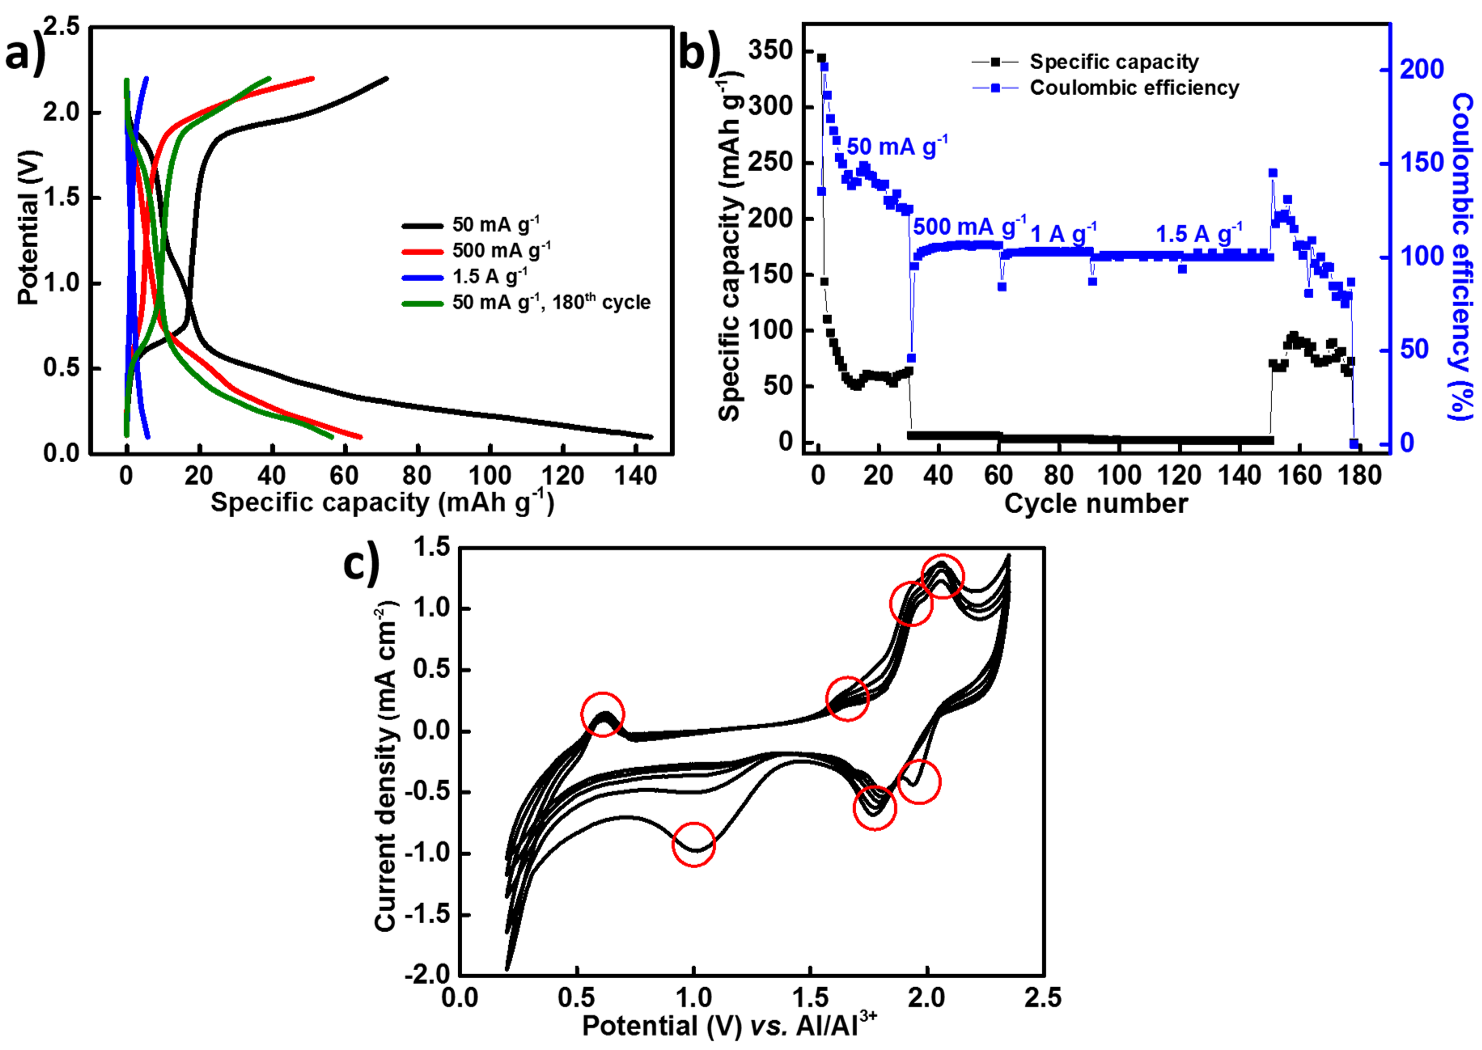
\includegraphics[width=\textwidth]{Figures/chap6fig/pbcdccecv}
    \caption{Galvanostatic cycle test of an Al/\ce{C19Fe7N18}, Prussian blue, cell in a two-electrode setup at various current rates. b) Long-term cell stability test at various current rates ranging from 50 to 1500 mA g$^{-1}$. c) CV curve of an Al/PB cell at a scan rate of 10 mV s$^{-1}$. The plateaus observed during charge at 0.6 and 1.8 V are almost identical to the oxidation peaks at 0.65 and 1.8 V. Voltage bend at 1.8 V during discharge corresponds to the sharp reduction peak at 1.8 V. Another oxidation peak at 2.15 V with a shoulder at 2.0 V }
  \label{Figures/chap6fig:pbcdccecv}
\end{figure}

\subsection{Summary}
In other battery systems, it had been reported that due to structure degradation, MOFs underwent large irreversible capacity losses and completed lesser number of cycles. This might be one of the reasons why the Al/MOF cell displayed a similar trend. However, Wang \ce{et al.} proposed a number of possible solutions to improve the performance of MOFs as a battery material. Supposing that the cell undergoes conversion-type reaction, the type of ligand in the MOF plays an important role because it determines if the MOF structure can be easily regenerated after every cycle. In case the cell undergoes an intercalation-type mechanism, MOF with a robust structure is highly desirable. A metal ion with multiple valence states and low molecular weight ligands rich in functional groups promotes insertion of \ce{Li+} ions \cite{wang_metalorganic_2016}. Therefore, altering the current MOF i.e. \ce{C19Fe7N18}, using the above-mentioned techniques would certainly improve its performance in AIBs. 

\section{Future developments}
\begin{itemize}
\item  In this chapter nanostructured cathode materials, owing to their special properties such as high surface area and ability to provide shorter ion diffusion path lengths, were tested as cathodes for non-aqueous AIBs. It was found that the performance of molybdenum dichalcogenide nanoflowers was not significantly different from the bulk. Similar battery voltages were observed for both bulk and nano-\ce{MoSe2}. Where bulk-\ce{MoSe2} displayed a capacity of $\sim$80mAh g$^{-1}$, \ce{MoSe2} nanoflowers displayed a capacity of <60 mAh g$^{-1}$ after 10 cycles with rapid capacity decay. Modifications can be made by increasing the number of layers present in nano-\ce{MoX2}, this might improve their performance and retain higher amounts of charge after every cycle.  
\item Another solution would be redesigning \ce{SnO2} fibers using materials that might make it more robust and eventually solve its problem of poor capacity retention. It is suggested that mixing the active material with carbon-based materials or making \ce{SnO2} hybrids (as suggested above for other battery systems) might improve the battery voltage. Like other battery systems, altering the structure of Prussian blue and g-\ce{C3N4} by adding suitable ligands will enhance the battery performance by achieving higher voltages and capacities. 
\end{itemize}

Supplemental research is required for an in-depth analysis of all the above-mentioned materials so that a comparative study can be made and a post-mortem analysis would also help in determining their individual mechanism. The current chapter makes way for a number of future projects in the field of AIBs, which will help in discovery of many more cathode materials for AIBs.  